\documentclass[uplatex,dvipdfmx,a4paper,11pt]{jsarticle}
%
% 数式
\usepackage{amsmath,amsthm,amssymb}
\usepackage{bm}
% 画像
\usepackage{graphicx}
%
\usepackage{multirow}
\usepackage{wrapfig}
\usepackage{ascmac}
\usepackage{xcolor}

\graphicspath{{../figures/}}

% ページ設定
% \pagestyle{empty}
% 高さの設定
\setlength{\textheight}{\paperheight}   % ひとまず紙面を本文領域に
\setlength{\topmargin}{-5.4truemm}      % 上の余白を20mm(=1inch-5.4mm)に
\addtolength{\topmargin}{-\headheight}  % 
\addtolength{\topmargin}{-\headsep}     % ヘッダの分だけ本文領域を移動させる
\addtolength{\textheight}{-40truemm}    % 下の余白も20mmに%% 幅の設定
\setlength{\textwidth}{\paperwidth}     % ひとまず紙面を本文領域に
\setlength{\oddsidemargin}{-5.4truemm}  % 左の余白を20mm(=1inch-5.4mm)に
\setlength{\evensidemargin}{-5.4truemm} % 
\addtolength{\textwidth}{-40truemm}     % 右の余白も20mmに
% 図と本文との間
%\abovecaptionskip=-5pt
%\belowcaptionskip=-5pt
%
% 全体の行間調整
% \renewcommand{\baselinestretch}{1.0} 
% 図と表
%\renewcommand{\figurename}{Fig.}
%\renewcommand{\tablename}{Tab.}


% \usepackage{makeidx}
% \makeindex

% \usepackage{qrcode}
% \setlength\lineskiplimit{0pt}
% \setlength\normallineskiplimit{0pt}

% \usepackage{qexam}

% \usepackage{titlesec}
% \titleformat*{\section}{\Large\bfseries}
% \titleformat*{\subsection}{\large\bfseries}
% \titleformat*{\subsubsection}{\normalsize\bfseries}
% \titleformat*{\paragraph}{\normalsize\bfseries}

\usepackage[dvipdfmx,%
 bookmarks=true,%
 bookmarksnumbered=true,%
 colorlinks=false,%
 setpagesize=false,%
 pdftitle={熱力学の基礎的事項},%
 pdfauthor={佐々木裕},%
 pdfsubject={},%
 pdfkeywords={熱力学; 演習; }]{hyperref}
\usepackage{pxjahyper}



%微分関連のマクロ
\newcommand{\diff}{\mathrm d}
\newcommand{\difd}[2]{\dfrac{\diff #1}{\diff #2}}
\newcommand{\difp}[2]{\dfrac{\partial #1}{\partial #2}}
\newcommand{\difdd}[2]{\dfrac{\diff^2 #1}{\diff #2^2}}
\newcommand{\difpp}[2]{\dfrac{\partial^2 #1}{\partial #2^2}}
%
%数式の途中で改行
\allowdisplaybreaks[3]


\title{熱力学の基礎的事項}
\author{佐々木裕}
\date{\today}

\setcounter{tocdepth}{4}

\begin{document}
\maketitle

%\begin{abstract}
%\end{abstract}
%\newpage

\pagenumbering{roman}
\tableofcontents
\newpage

\setcounter{secnumdepth}{4}
\pagenumbering{arabic}


%%%%%%%%%%
%%% はじめに
%%%%%%%%%%
\section*{はじめに}

熱力学とは、「熱」と「仕事」を対象として、それらの関係を明らかにすることで、自然現象の成り立ちを明らかにする学問である。
これは、これまでの経験に基づいて確かめられてきている少数の{\bf「普遍的法則」}を基とし、それらを{\bf「公理として構成された論理的な閉じた体系」}である 。

このメモでは、統計力学を理解するために最低限必要となる程度の、熱力学に関する基礎的な事項について、できるだけ簡単にまとめた。
そのため、エントロピーの導出等の、熱力学のもっとも理解しにくいような部分に関する記述は大幅に省略している。

熱力学は、基本的には、系の平衡状態について議論を進めるものである。
したがって、系の平衡状態の指標となる「熱力学ポテンシャルの概念」を理解することがもっとも重要である。

熱力学ポテンシャルの理解するための考え方の流れを図 \ref{fig:flow} に示した。

\begin{figure}[htbp]
\centering
	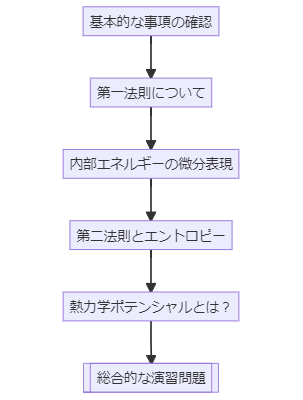
\includegraphics[width=.7\textwidth]{flow.png}
\caption{熱力学ポテンシャルを理解するための考え方の流れ}\label{fig:flow}
\end{figure}

\newpage

%%% 2
\section{基礎的用語}

\subsection{熱と仕事}
%この項目に関連する事項を、以下に整理した。

\begin{description}
\item[温度]
暑いとか寒いという寒暖の感覚を定量的に表すものであり高い(大きい)方には制限がないが、低いほうには限度(絶対零度: $0K = -273.15 {}^\circ {\rm C}$)がある。

\item[熱]
物体の温度を変化させる原因を、「熱」とよぶ。
高温の物体と低温の物体を接触させると、前者の温度は低下し後者は高温になり、高温物質から低温物質に熱が移動したという。

すでに否定された考え方であるが、カルノーも当初賛同したカロリック(熱素)というような伝達体が移動すると考えたほうが理解しやすいかもしれない。

分子運動論的な考え方を利用すると、接触する二つの系のそれぞれの系中の分子の運動エネルギーの平均に差があった場合、その差が減少し均一になるように運動エネルギーが分配される過程が、熱の移動であるととらえることができる。

\item[熱量]
熱を数量的に表したものであり、$Q$ と書く場合が多い。
$1$ g の水の温度を $1$ K だけ上げるのに必要な熱量を、$1$ カロリー(cal)という。

\item[熱容量]
ある物体の温度を 1 K だけ上げるのに必要な熱量 $Q$ を、その物体の「熱容量 $C$ [cal/K or J/K]」という。

系がある準静的な過程で $\Delta Q$ の熱を得たとき、温度が $\Delta T$ 変化したとすると、熱容量は
\[C = \dfrac{\Delta Q}{\Delta T}\]
で定義される。 

\item[比熱]
単位量の任意の物質の温度を 1 K だけ上げるのに必要な熱量を、すなわち、単位量当た値の熱容量を、その物質の「比熱 $c$」と呼ぶ。
一般には、単位量としては 1 g あたりを考えて [cal/g$\cdot$K or J/g$\cdot$K] とする。

\item[モル比熱]
熱力学では単位量としてモルを考える場合が多い。
1 モルの物質が持つ熱容量を、その物質の「モル比熱 [cal/mol $\cdot$K or J/mol $\cdot$K]」という。

\begin{description}
\item[定積モル比熱]
体積を一定に保つ場合のモル比熱であり、定積条件下で物質 1 モルの温度を 1 K 増加させるために必要な熱量のことである。
物質のモル数を n モルとし、熱量を $Q$ で表した場合、以下のように定義される。
\begin{equation*}
C_V = \dfrac{1}{n} \left( \dfrac{\partial Q}{\partial T} \right)_V
\end{equation*}

\item[定圧モル比熱]
圧力を一定に保つ場合のモル比熱であり、定圧条件下で物質 1 モルの温度を 1 K 増加させるために必要な熱量のことである。
\begin{equation*}
C_P = = \dfrac{1}{n} \left( \dfrac{\partial Q}{\partial T} \right)_P
\end{equation*}
理想気体の場合は以下に示したマイヤーの関係が成立する。
\begin{equation*}
C_P - C_V = R
\end{equation*}


\end{description}


\item[熱の仕事当量]
熱量($Q$)は力学的仕事($W$)と等価で、この比例係数が熱の仕事当量($J=4.19$ [J/cal])であり、両者の関係は以下となる。
\begin{equation*}
W=4.19 Q
\end{equation*}

\item[熱量保存の法則]

外部との間に熱の出入りがないようにして温度の異なる二つの物質を接触、あるいは、混合した場合に成り立つ以下の関係を「熱量保存の法則」と呼ぶ。
\begin{equation*}
\text{高温物質の失った熱量} = \text{低温物質が得た熱量}
\end{equation*}

\end{description}

\subsection{系の変化}
%この項目に関連する事項を、以下に整理した。
\begin{description}
\item[系]
熱力学の考察の対象となるものであり、系以外の残りの部分は外界と呼ばれる。

外界との関係性から、以下の様に三つに分類される。
なお、系を入れ子に設定することもできる。

\begin{description}
\item[解放系]
外部との間で、何でも交換できる系。
\item[閉鎖系]
外部との間でエネルギー(あるいは熱)は交換できるが、物質は交換できない系。
\item[孤立系]
外界との熱および物質のやり取りを遮断された、体積一定の系。
\end{description}

\item[過程]
系の状態を、ある熱平衡状態から、別の熱平衡状態へと変化させる途中のことを指す。

\begin{description}
\item[可逆過程]
ある変化をさせた後でも、何らかの方法で、外界への影響も含めて完全に元の状態に戻すことができるような変化の過程。

\item[不可逆過程]
如何なる方法をもってしても、{\bf 完全には元の状態(含、外界への影響)には戻せなくなるような変化}の過程。

\item[準静的過程]
変化の各瞬間において、系および外界が常に平衡状態にあると仮定できる程度に変化がゆっくりしており、かつ、平衡からのずれが各瞬間で無視できる程度に小さい状態を保ちながら変化を行う過程。
\end{description}

\end{description}

\subsection{状態量と状態方程式}
%この項目に関連する事項を、以下に整理した。
\begin{description}
\item[状態]
「系の在りよう」のことである。
\footnote
{
熱力学が対象とする系においては、比較的少数の変数により系の状態が決定できる事が特徴的である。
この事実は、熱力学が対象とする巨視的な状態が、非常に大多数の分子の運動の平均値として記述されるため、平均値まわりのゆらぎが無視できるようになっているためであると考えることができる。
}

\item[平衡状態]
孤立系を充分に長い時間放置した時に、系の内部が一様と見なせるようになって巨視的な変化が生じなくなった状態。
簡単に言えば、「それ以上に自発的な変化が生じない状態」のことである。

\item[熱平衡]
二つの物体があり、それらの温度が等しく、両物体の間に熱の移動がないとき、この二つの物体は「熱平衡」の状態にあるという。

\item[熱力学的状態量]
系の過去の変化の経路には依存することなく、系が置かれている熱力学的状態のみによってその値が決まる量。

\begin{description}
\item[示強性状態量]
系の大きさに因らない状態量であり、温度、圧力、密度、濃度等がある。
\item[示量性状態量]
系の大きさに比例する状態量であり、体積、質量、エネルギー、エントロピー等が挙げられる。
\end{description}

\item[状態方程式]
熱平衡にある均質な系において、状態量の間に成立する方程式のこと。
たとえば、理想気体の場合、温度 $T$ と体積 $V$ を決めると圧力 $P$ も決まるというボイル・シャルルの法則が知られており、以下のように書ける。
\begin{equation*}
PV = nRT
\end{equation*}
ただし、$n$ は、気体のモル数、$R$ は気体定数である。

\end{description}

\newpage

\subsection{演習問題}


\begin{enumerate}
\item
{\bf (基本的な用語)}

以下のそれぞれの用語の意味を説明せよ。なお、関連性のある事項については、それについても言及せよ。

\begin{enumerate}
\item
熱

%{\bf 解答例}
%物体の温度を変化させる原因を、「熱」とよぶ。
%高温の物体と低温の物体を接触させると、前者の温度は低下し後者は高温になり、高温物質から低温物質に熱が移動したという。

\item
熱量
%
%{\bf 解答例}
%
%熱を数量的に表したものであり、$Q$ と書く場合が多い。
%$1$ g の水の温度を $1$ K だけ上げるのに必要な熱量を、$1$ カロリー(cal)という。

\item
熱容量
%
%{\bf 解答例}
%
%ある物体の温度を 1 K だけ上げるのに必要な熱量 $Q$ を、その物体の「熱容量 $C$ [cal/K or J/K]」という。
%
%系がある準静的な過程で $\Delta Q$ の熱を得たとき、温度が $\Delta T$ 変化したとすると、熱容量は
%\[C = \dfrac{\Delta Q}{\Delta T}\]
%で定義される。 

\item
比熱

%{\bf 解答例}
%
%単位量の任意の物質の温度を 1 K だけ上げるのに必要な熱量を、すなわち、単位量当た値の熱容量を、その物質の「比熱 $c$」と呼ぶ。
%一般には、単位量としては 1 g あたりを考えて [cal/g$\cdot$K or J/g$\cdot$K] とする。
%
%\begin{description}
%\item[モル比熱]
%1 モルの物質が持つ熱容量を、その物質の「モル比熱 [cal/mol $\cdot$K or J/mol $\cdot$K]」という。
%
%\item[定積モル比熱]
%体積を一定に保つ場合のモル比熱であり、定積条件下で物質 1 モルの温度を 1 K 増加させるために必要な熱量のことである。
%物質のモル数を n モルとし、熱量を $Q$ で表した場合、以下のように定義される。
%\begin{equation*}
%C_V = \dfrac{1}{n} \left( \dfrac{\partial Q}{\partial T} \right)_V
%\end{equation*}
%
%\item[定圧モル比熱]
%圧力を一定に保つ場合のモル比熱であり、定圧条件下で物質 1 モルの温度を 1 K 増加させるために必要な熱量のことである。
%\begin{equation*}
%C_P = = \dfrac{1}{n} \left( \dfrac{\partial Q}{\partial T} \right)_P
%\end{equation*}
%理想気体の場合は以下に示したマイヤーの関係が成立する。
%\begin{equation*}
%C_P-C_V = R
%\end{equation*}
%
%\end{description}
%

\item
熱の仕事当量

%{\bf 解答例}
%
%熱量($Q$)は力学的仕事($W$)と等価で、この比例係数が熱の仕事当量($J=4.19$ [J/cal])であり、両者の関係は以下となる。
%\begin{equation*}
%W=4.19 Q
%\end{equation*}

\item
系

%{\bf 解答例}
%
%熱力学の考察の対象となるものであり、系以外の残りの部分は外界と呼ばれる。
%
%外界との関係性から、以下の様に三つに分類される。
%なお、系を入れ子に設定することもできる。
%
%\begin{description}
%\item[解放系]
%外部との間で、何でも交換できる系。
%\item[閉鎖系]
%外部との間でエネルギー(あるいは熱)は交換できるが、物質は交換できない系。
%\item[孤立系]
%外界との熱および物質のやり取りを遮断された、体積一定の系。
%\end{description}

\item
熱力学的状態量

%{\bf 解答例}
%
%系の過去の変化の経路には依存することなく、系が置かれている熱力学的状態のみによってその値が決まる量。
%
%\begin{description}
%\item[示強性状態量]
%系の大きさに因らない状態量であり、温度、圧力、密度、濃度等がある。
%\item[示量性状態量]
%系の大きさに比例する状態量であり、体積、質量、エネルギー、エントロピー等が挙げられる。
%\end{description}

\end{enumerate}

\item
{\bf (温度変化)}

\begin{enumerate}
\item
滝の頂部で水の温度が 283 K (= 10.0${}^\circ$C) であった。
水が 50.0 m 落下したとき、そのすべての運動エネルギーが水の加熱に使われると仮定すると滝の底に落ちた水の温度は何 K 上昇するか?
ただし、重力加速度を 9.80 m/${\rm s}^2$、熱の仕事当量を 4.19 kJ/kgK とする。

%{\bf (解答例)}
%
%単位量の水(1.00 kg)を考える。
%水の落下によってなされる仕事は、水の落下により得る運動エネルギーと考えることができ、これは、落下前の位置エネルギーに等しいので、
%\begin{equation*}
%W = mgh = 1.00 \times 9.80 \times 50.0 = 490 J = 0.490 kJ
%\end{equation*}
%
%この仕事で得たエネルギーが水の温度上昇に使われるので、温度上昇を $\Delta T$ とすると、
%\begin{equation*}
%\Delta T = \dfrac{0.490}{4.19} = 0.120 K
%\end{equation*}。

\item
283 K の水 5.00 kg を 273 K の水 2.50 kg と混合する。
この系の最終温度 $T$ は何 K になるか?

%{\bf (解答例)}
%
%それぞれの水が最終温度に変化した場合の熱量変化が等しいとして、
%\begin{align*}
%(283 - T) \times 5.00 &= (T - 273) \times 2.50 \\
%283\times5.00 - 5.00 T &=  -273\times2.50 + 2.50 T \\
%7.50T &= 1415 + 683 = 2098 \\
%T &= 280 K
%\end{align*}

\item
283 K の水 5.00 kg を 273 K の氷 2.50 kg に加える。
この系の最終温度 T は何 K になるか?
もし、T = 273 K ならば、どれだけの氷が残っているか?
なお、氷の融解熱は 333 kJ/kg とせよ。

%{\bf (解答例)}
%
%まず、氷の融解に必要な熱量 $Q_{melt}$ を確認する。
%\begin{equation*}
%Q_{melt} = 2.50 \times 333 = 833 {\rm kJ}
%\end{equation*}
%
%一方、283 K の水 5.00 kg を 273 K にした場合に失う熱量は、
%\begin{equation*}
%(283 - 273) \times 5.00 \times 4.19 = 210 {\rm kJ}
%\end{equation*}
%したがって、この二つを混合しても氷を全部溶かすことはできないので、混合物の最終温度T = 273 K となる。
%
%このとき、氷の残量を $x$ kg とすると、上記の 283 K の水が失った熱量が氷の溶解に使われるので、
%\begin{align*}
%(2.50 - x) \times 333 &= 210 \\
%333 x &= 833 - 210 \\
%x &= \dfrac{623}{333} \\
%	& = 1.87 {\rm kg}
%\end{align*}

\end{enumerate}


\item 
{\bf (気体の仕事)}

\begin{enumerate}
\item
ピストンつきシリンダ中に、300 K で 0.200 L (= 0.200 $\times 10^{-3} {\rm m}^3$) の空気を封入した。
圧力を1気圧($1.01 \times 10^5 {\rm N}/{\rm m}^2$)に保ったまま 330 K まで暖めると、体積はいくらになるか。
また、このとき空気のする仕事はいくらか?

%{\bf (解答例)}
%
%変化後の体積を V としたとき、ボイル・シャルルの法則から、
%\begin{equation*}
%V = 0.200 \times 10^{-3} \times \dfrac{330}{300} = 0.200 \times 1.1 \times 10^{-3} = 0.220 \times 10^{-3} {\rm m}^3
%\end{equation*}
%
%
%圧力に抗してピストンを移動させるのであるから、この時の仕事 $W$ は、
%\begin{align*}
%W &= P \Delta V \\
%	&= 1.01 \times 10^5 \times \{ (0.220 - 0.200) \times 10^{-3} \} \\
%	&= 1.01 \times 0.020 \times 10^{2} = 2.02 {\rm J}
%\end{align*}

\item
0.0100 L (= 0.0100 $\times 10^{-3} {\rm m}^3$) の水が 16.7 L の水蒸気になった。
このとき水蒸気のする仕事はいくらか。
ただし圧力を1気圧($1.01 \times 10^5 {\rm N}/{\rm m}^2$)とする。

%{\bf (解答例)}
%
%水蒸気になったものの体積変化だけを考えればよいので、この時の仕事 $W$ は、
%\begin{align*}
%W &= P \Delta V \\
%	&= 1.01 \times 10^5 \times \{ (16.7 - 0.010) \times 10^{-3} \} \\
%	&= 1.01 \times 16.7 \times 10^{2} = 1.69 {\rm kJ}
%\end{align*}

\end{enumerate}


\end{enumerate}

\newpage

%%%%%%
%% Sec. 2
%%%%%%

\section{熱力学の第一法則}
熱力学の第一法則は、「系と外界を合わせた全エネルギーは一定不変である」というエネルギー保存則である。
系のエネルギーは後述の内部エネルギーで表されるので、「内部エネルギーの変化量が外界とのエネルギーのやり取りと等しい」ということを示す法則である。

\subsection{内部エネルギーと外界との釣り合い}

\subsubsection{内部エネルギー}
内部エネルギーとは系を構成する物質が持つあらゆるエネルギーの総和であって、熱エネルギー(運動エネルギー)、ポテンシャルエネルギー、化学結合エネルギー、分子間相互作用エネルギー等々の、ありとあらゆるものが含まれる{\bf 示量性状態量}である。

ただし、熱力学では系の状態変化のみを取り扱うわけであるから、状態変化に伴って変化するエネルギーのみを内部エネルギーに含め、変化しないエネルギーは対象外とする。
したがって、比較する二つの状態において分子構造の変化がない場合には、化学結合エネルギー等は考慮する必要がなくなる。
%さらに、理想気体を対象とすると、内部エネルギーは温度のみ(体積に依存しない)の関数となる。


\subsubsection{内部エネルギーと外界との釣り合い}
$i = A, B, C, \cdots$ で指定される複数の成分からなり、内部エネルギーが $E_1$ である系に対して、外界から、熱量 $\Delta Q$、仕事 $\Delta W$ そして、$i$ 種の粒子 $\Delta N_i$ を流入させたときに、内部エネルギーが $E_2$ へと変化したとする。

これを数式で書けば、
\begin{equation}
E_2 = E_1 + \Delta Q + \Delta W + \sum_i \mu_i \Delta N_i
\end{equation}
であるから、内部エネルギーの変化量 $\Delta E$ を第一法則に従って表すと、
\begin{equation}
\Delta E = E_2 -E_1 = \Delta Q + \Delta W + \sum_i \mu_i \Delta N_i
\end{equation}
となり、系が外界とやり取りしたエネルギー量の差分(熱量 $\Delta Q$、仕事 $\Delta W$ および$\sum_i \mu_i \Delta N_i$)が、内部エネルギー変化量 $\Delta E$ と等しい、すなわち、系と外界とを合わせればエネルギー総量には、変化がないということになる。

混乱しがちな仕事の符号について、再度、確認しておこう。
ここまでに示してきたものは、{\bf 「外界から流入してきたものを正」}としている。
したがって、系が外界に対して仕事をした場合には、その符号を、マイナスとすることになり、内部エネルギーを表す式も以下となる。

\begin{equation*}
\Delta E = \Delta Q - \Delta W + \sum_i \mu_i \Delta N_i \quad \text{(外界に仕事をした場合)}
\end{equation*}

\subsubsection{微小変化の場合の表式}
つぎに、この変化が無限小である場合を考えよう。

繰り返しになるが、内部エネルギーは状態量であるから、系の過去の変化の経路に依存することなく現在の状態だけで決まる値である。
また、粒子の数も状態量である。
したがって、これら2つの因子については、{\bf その微小量変化も経路に依存することなく一義に決まるので、数学的な全微分として取り扱う}ことができる。
このことを明示するために、記号 $d$ により熱力学的状態量に対する無限小変化を表すことにする。

一方、熱量や仕事は状態量ではなく、変化の経路に依って決まる値なので、無限小変化を表現する場合にもその経路を考慮する必要がある。
状態量ではない物理量の無限小変化を全微分と区別して表すために、記号 $d'$ を用いることとする。

したがって、系の内部エネルギーの微小変化は、微分表現の形で以下のように書くことができる。
\begin{equation}
\diff E = \diff' Q + \diff' W + \sum_i \mu_i \diff N_i
\label{eq:1st_low}
\end{equation}


\subsection{熱力学第一法則の全微分表現}
全微分ではない、仕事および熱の微小変化を、全微分の形に変形することを考えよう。

準静的過程とは、変化の各瞬間において系および外界が常に平衡状態にあると仮定できる程度に変化をゆっくり行い、平衡からのずれが各瞬間で無視できる程度に小さい状態として変化を行う過程であった。このような過程を想定することで、熱力学第一法則を全微分の形で表記することができる。

\subsubsection{純静的過程での仕事}
単純化した問題とするために、対象とする系が「シリンダーの中に気体を入れてピストンで蓋をした」ようなものであるとしよう。
そして、シリンダー内部の気体の圧力 $P$ と外部からの圧力が釣り合うようにピストンを準静的に移動させる「準静的過程」でピストンの位置を $\Delta x$ 移動させ、系の体積を $\Delta V$ だけ変化(膨張)させることを考える。

この時、ピストンに加える力を $F$ とすると、$P = \dfrac{F}{A}$($A$ はピストンの断面積)であるので、シリンダー内部の気体が外界になす仕事 $- \Delta W$ は
\footnote
{
なお、系が外界に対して仕事をなすわけであるので、符号はマイナスとなる。
}、
\begin{align}
	-\Delta W 
		&= F \times \Delta x \notag \\
		&= (P \times A) \times \Delta x \notag \\
		&= P \times (A \times \Delta x) \notag \\
		&= P \times \Delta V
\end{align}
となる。


したがって、(\ref{eq:1st_low})式においては、$\diff' W = -P \diff V$ となり、仕事を示量性状態量 $V$ の全微分 $\diff V$ を用いて書けることになる。

\subsubsection{エントロピーの導入}

一方、熱の移動 $\diff' Q$ も非状態量であるが、上述のような、非常にゆっくりとした変化である準静的過程においては、積分因子
\footnote
{
積分因子とは、不完全微分に掛けることにより、完全微分を得ることのできる因子であり、常に存在するとは限らないが、二変数の方程式の場合には、積分因子は常に存在する。
} $1/T$ を用いて、
\begin{equation}
\diff S = \dfrac{\diff' Q}{T}
\end{equation}
とすることで、全微分形式に書き直すことが可能である。

このようにして定義された熱力学量 $S$ は状態量であり、エントロピーと呼ばれる
\footnote
{
このエントロピーの導出は、熱力学を納得して理解するために重要であるが、ここではその説明は省略する。
必要に応じて、教科書を参照していただきたい。
}。

\subsubsection{第一法則の全微分表現}

このエントロピーの定義を用いれば、熱力学第一法則は、全微分の形で、
\begin{equation}
\diff E = T \diff S - P \diff V + \sum_i \mu_i \diff N_i \quad \text{(準静的変化の場合)}
\label{eq:1st_low_der}
\end{equation}	
と書き換えられる。

したがって、内部エネルギーの全微分表現 $\diff E$ は、示強性変数である温度 $T$、圧力 $P$、化学ポテンシャル $\mu_i$ と、示量性変数であるエントロピー $S$、体積 $V$ および粒子数 $\{ N_i \}$ の全微分との積の形で記述できることになる。
\newpage

\subsection{演習問題}


\begin{enumerate}
\item
{\bf (基本的な用語)}

以下のそれぞれの用語の意味を説明せよ。なお、関連性のある事項については、それについても言及せよ。

\begin{enumerate}

\item
内部エネルギー

%{\bf (解答例)} 
%
%内部エネルギーとは系を構成する物質が持つあらゆるエネルギーの総和であって、熱エネルギー(運動エネルギー)、ポテンシャルエネルギー、化学結合エネルギー、分子間相互作用エネルギー等々の、ありとあらゆるものが含まれる{\bf 示量性状態量}である。
%ただし、熱力学では系の状態変化のみを取り扱うわけであるから、状態変化に伴って変化するエネルギーのみを内部エネルギーに含め、変化しないエネルギーは対象外とする。
%
%したがって、比較する二つの状態において分子構造の変化がない場合には、化学結合エネルギー等は考慮する必要がなくなる。
%さらに、理想気体を対象とすると、内部エネルギーは温度のみ(体積に依存しない)の関数となる。

\item
熱力学の第一法則

%{\bf (解答例)} 
%
%熱力学の第一法則は、「系と外界を合わせた全エネルギーは一定不変である」というエネルギー保存則である。
%
%例えば、内部エネルギーが $E_1$ である単一成分からなる系に対して、外界から、熱量 $\Delta Q$、仕事 $\Delta W$ を流入させたときに、内部エネルギーが $E_2$ へと変化したする。
%第一法則より、系と外界とを合わせればエネルギー総量に変化がないので、系が外界とやり取りしたエネルギー量の差分(熱量 $\Delta Q$、仕事 $\Delta W$)が、内部エネルギー変化量 $\Delta E$ と等しいことになり、
%\begin{equation*}
%\Delta E = E_2 -E_1 = \Delta Q + \Delta W
%\end{equation*}
%となる。
%
%なお、上記表現は、{\bf 「外界から流入してきたものを正」}としているので、系が外界に対して仕事をした場合には、その符号をマイナスとし、内部エネルギーを表す式は以下となる。
%\begin{equation*}
%\Delta E = \Delta Q - \Delta W \quad \text{(外界に仕事をした場合)}
%\end{equation*}

\item
エントロピー

%{\bf (解答例)} 
%
%エントロピー $S$ は示量性状態量である。
%
%その定義は、以下であり、
%\begin{equation*}
%\diff S = \dfrac{\diff' Q}{T}
%\end{equation*}
%これは、孤立系における準静的な可逆過程においては、途中経過に依存する非状態量である熱量の変化 $\diff' Q$ が積分因子 $1/T$ を用いることで、全微分形式の状態量であるエントロピーに書き直すことができることを表している。

\end{enumerate}


\item
{\bf (内部エネルギー)}

\begin{enumerate}
\item
0.0100 kg、0.0100 L の水に1気圧($1.01 \times 10^5 {\rm N}/{\rm m}^2$)のもとで、10.0 kJ の熱を加えたところ、16.7 L の水蒸気になった。
内部エネルギーはいくら増加したか。

%{\bf (解答例)}
%
%外界に対して水蒸気がなした仕事は、上記の解答例から、$W=1.69$ kJ である。
%したがって、内部エネルギーの変化量 $\Delta E$ は、
%\begin{equation*}
%\Delta E = Q - W = 10.0 - 1.69 = 8.31 {\rm kJ}
%\end{equation*}

\item
左右に自由に移動できるピストン(断面積が $S$ [${\rm m}^2$])を一定の力 $f$ [N] で保持することで、シリンダー中に $n$ モルの理想気体が封入されている。
気体の初期状態は、体積 $V$ [${\rm m}^3$]、温度 $T$ [K] であった。
外部から熱を加えて、気体の温度を $T$ から $T'$ に上げた時、内部エネルギーはどのように変化するか?

ただし、気体の定圧モル比熱を $C_P$ とし、温度依存性は無視する。
さらに、容器に関係する熱量変化も無視する。

%{\bf (解答例)}
%
%断面積が $S$ のピストンを一定の力 $f$ で保持するということは、圧力 $P= \dfrac{f}{S}$ を維持することに対応し、この状態で気体の温度を $T$ から $T'$ に上げた時の体積変化 $\Delta V$ は、ボイル・シャルルの法則から、
%\begin{align*}
%V + \Delta V &= V \dfrac{T'}{T} \\
%\Delta V &= V\dfrac{T' - T}{T} 
%\end{align*}
%このとき、温度上昇によって気体が外界になす仕事 $W$ は、
%\begin{equation*}
%W = -P\Delta V =- \dfrac{f}{S} V\dfrac{T' - T}{T}
%\end{equation*}
%
%一方、温度上昇に伴い受け入れた熱量は、
%\begin{equation*}
%Q = n C_P \Delta T
%\end{equation*}
%したがって、内部エネルギー増加量 $\Delta E$ は、
%\begin{equation*}
%\Delta E = Q + W = n C_P \Delta T - \dfrac{f}{S} V\dfrac{T' - T}{T}
%\end{equation*}

\end{enumerate}

\item
{\bf (内部エネルギーの微分表現)}

\begin{enumerate}
\item
$i = A, B, C, \cdots$ で指定される複数の成分からなり、内部エネルギーが $E_1$ である系に対して、外界から、熱量 $\Delta Q$、仕事 $\Delta W$ そして、$i$ 種の粒子 $\Delta N_i$ を流入させたときの内部エネルギーの変化量 $\Delta E$ を第一法則に従って表せ。

%{\bf (解答例)} 
%
%熱力学の第一法則に従えば、「系と外界とを合わせればエネルギー総量には、変化がない」のであるから、「系が外界とやり取りしたエネルギー量の差分(熱量 $\Delta Q$、仕事 $\Delta W$ および$\sum_i \mu_i \Delta N_i$)が、内部エネルギー変化量 $\Delta E$ と等しい」ことになる。
%
%内部エネルギーが $E_2$ へと変化したとすると、内部エネルギーの変化量 $\Delta E$ は、
%\begin{equation*}
%\Delta E = E_2 -E_1 = \Delta Q + \Delta W + \sum_i \mu_i \Delta N_i
%\end{equation*}
%となる。

\item
準静的過程で系が変化したものとして、上記の内部エネルギーを全微分形式で表せ。

%{\bf (解答例)} 
%
%前問の解答における変化が無限小であると考え微分形式で記述すれば、
%\begin{equation*}
%\diff E = \diff' Q + \diff' W + \sum_i \mu_i \diff N_i
%\end{equation*}
%
%内部エネルギー、および、粒子の数は状態量であり、経路に依存することなく一義に決まるので、数学的な全微分として記号 $d$ により熱力学的状態量に対する無限小変化を表せる。
%一方、熱量や仕事は状態量ではなく、変化の経路に依存するため全微分と区別して表すために、記号 $d'$ を用いている。
%
%ここで、一定圧力 $P$ の下で準静的過程で系の体積が変化したと考えると、示量性状態量 $V$ の全微分 $\diff V$ と $P$ との積で仕事を表すことができる。
%
%一方、熱の移動 $\diff' Q$ のほうは非状態量であるが、準静的過程においては、積分因子 $1/T$ を用いて、
%\begin{equation*}
%\diff S = \dfrac{\diff' Q}{T}
%\end{equation*}
%とすることで、示量性状態量であるエントロピー $S$ の全微分形式に書き直すことが可能である。
%
%このエントロピーの定義を用いれば、熱力学第一法則は、全微分の形で、
%\begin{equation*}
%\diff E = T \diff S - P \diff V + \sum_i \mu_i \diff N_i \quad \text{(準静的変化の場合)}
%\end{equation*}	
%と書き換えられる。

\end{enumerate}

%\item 
%{\bf (定積モル比熱)}
%
%定積モル比熱が以下の式で定義されることを示せ。
%なお、$n$ は気体のモル量、$E$ は内部エネルギー、$T$ は絶対温度、$V$ は体積である。
%\begin{equation*}
%C_V = \dfrac{1}{n} \left( \dfrac{\partial E}{\partial T} \right)_V
%\end{equation*}
%
%%{\bf (解答例)}
%%
%%熱力学の第一法則より、
%%\begin{equation*}
%%\Delta E = \Delta Q - \Delta W  = \Delta Q - P\Delta V 
%%\end{equation*}
%%ここで、定積変化を考えるのであるから、$\Delta V = 0$、したがって、
%%\begin{equation*}
%%\Delta E = \Delta Q
%%\end{equation*}
%%
%%一方、定積モル比熱の定義は、「体積を一定に保つ場合のモル比熱であり、定積条件下で物質 1 モルの温度を 1 K 増加させるために必要な熱量」であり、
%%\begin{equation*}
%%\Delta Q = n \times C_V \times \Delta T 
%%\end{equation*}
%%
%%上に示した二つの式から、
%%\begin{align*}
%%n \times C_V \times \Delta T &=\Delta E \\
%%\therefore C_V &= \dfrac{1}{n} \left( \dfrac{\partial E}{\partial T} \right)_V
%%\end{align*}
%%
%%
%
%
%\item
%{\bf (理想気体)}
%
%\begin{enumerate}
%\item
%内部エネルギー
%
%理想気体の内部エネルギー $E$ が、体積 $V$ と温度 $T$ の関数 $E(V,T)$ であるとしたとき、これが、体積 $V$ に依存しないことを示せ。
%
%(ヒント)
%
%マックスウェルの関係式から、$\left(\dfrac{\partial S}{\partial V} \right)_T = \left(\dfrac{\partial P}{\partial T} \right)_V$ となることを利用する。
%
%%{\bf (解答例 1)}
%%
%%内部エネルギーが体積 $V$ に依存しないことを示すためには、内部エネルギーを体積で微分すれば 0 となることを示せばよい。
%%
%%内部エネルギーの全微分形式での表式は以下であった。
%%\begin{equation*}
%%\diff E = T \diff S -P \diff V
%%\end{equation*}
%%
%%上式は、以下のように変形できる。
%%\begin{align*}
%%\left(\dfrac{\partial E}{\partial V} \right)_T 
%%	&= T \left(\dfrac{\partial S}{\partial V} \right)_T -P \\
%%	&= T \left(\dfrac{\partial P}{\partial T} \right)_V -P \\
%%	&= T \left(\dfrac{\partial}{\partial T} \dfrac {nRT}{V} \right)_V -P \\
%%	&= T \left(\dfrac {nR}{V}\right) -P \\
%%	&= 0
%%\end{align*}
%%なお、二行目への展開では、マックスウェルの関係式から、$\left(\dfrac{\partial S}{\partial V} \right)_T = \left(\dfrac{\partial P}{\partial T} \right)_V$(後述の「マックスウェルの関係式」に関する問題を参照)であることを用い、三行目と四行目では、理想気体の状態方程式から、$P = \dfrac {nRT}{V}$ を利用した。
%%
%%上式に示したように、内部エネルギーの体積依存を表す $\left(\dfrac{\partial E}{\partial V} \right)_T = 0$ であるから、内部エネルギーは体積に依存しないことになる。
%%
%%{\bf (解答例 2)}
%%
%%気体分子の存在を認めた気体分子運動論の立場からの考え方も確認してみよう。
%%
%%気体が単原子分子から成り立っていると考えると、内部エネルギーは、並進運動に基づく分子の運動エネルギーと分子間力による位置エネルギーとの総和と考えることができる。
%%
%%理想気体においては、分子間力による位置エネルギーがないものとしているので、理想気体に存在するのは運動エネルギーのみとなる。
%%これらの運動エネルギーは、デカルト座標の各方向あたりに均等配分されるので、並進運動エネルギーに比例することになる。
%%気体分子運動論では、並進運動エネルギーが温度を決めるものであると考えているので、内部エネルギーも温度のみによって決まることになり、体積には依存しないことが確認できた。
%%
%%上記は、「分子間力による位置エネルギーは体積に応じて変化するが、それが、理想気体には存在しないため」と言い換えることもできる。
%
%\item
%定積モル比熱の体積依存
%
%定積モル比熱 $C_V = \dfrac{1}{n} \left( \dfrac{\partial E}{\partial T} \right)_V$ が温度のみの関数であり、体積には依存しないことを示せ。
%
%%{\bf (解答例)}
%%
%%前門と同様に、定積モル比熱が体積 $V$ に依存しないことを示すためには、定積モル比熱を体積で微分すれば 0 となることを示せばよい。
%%
%%具体的に偏微分を行い、
%%\begin{align*}
%%\difp{}{V} C_V 
%%	&=\difp{}{V} \dfrac{1}{n} \left( \dfrac{\partial E}{\partial T} \right)_V \\
%%	&=\dfrac{1}{n} \difp{}{T} \left( \difp{E}{V} \right)_T \\
%%	&=\dfrac{1}{n} \difp{}{T} (0) \\
%%	&= 0
%%\end{align*}
%%なお、二行目へは内部エネルギーが状態量であることから $\difp{}{V} \left( \dfrac{\partial E}{\partial T} \right)_V=\difp{}{T} \left( \difp{E}{V} \right)_T$ のように偏微分の順番を入れ替えられることを用いている。
%
%\item
%理想気体のエントロピー
%
%理想気体の物質量が 1 モル、温度 $T$、体積 $V$ の場合、そのエントロピー $S$ が次のように表されることを、熱力学第一法則、理想気体の性質などを用いて導け。
%\[S = C_V \ln T + R \ln V + const. \]
%
%%{\bf (解答例)}
%%
%%前問題の結果より、定積モル比熱は体積には依存しないので、定義式 $C_V = \dfrac{1}{n} \left( \dfrac{\partial E}{\partial T} \right)_V$ を積分して、
%%\begin{align*}
%%E= C_V T + const.
%%\end{align*}
%%である。
%%この関係と理想気体の状態方程式 $PV = RT$ を、熱力学第一法則の保存式に用いて、
%%\begin{align*}
%%\diff E &= d' Q − P \diff V \\
%%\therefore \quad d' Q 
%%	&= \diff E + P \diff V \\
%%	&= C_V \diff T + RT \dfrac{\diff V}{V}
%%\end{align*}
%%を得る。
%%これを、エントロピー(変化)の定義に代入して、
%%\begin{align*}
%%dS 
%%	&= \dfrac{d' Q}{T} \\
%%	&= C_V \dfrac{\diff T}{T} + R \dfrac{\diff V}{V}
%%\end{align*}
%%
%%両辺を積分することで、理想気体のエントロピーの表式として、
%%\begin{align*}
%%S = C_V \ln T + R \ln V + const.
%%\end{align*}
%%を得る。
%%
%
%\item
%断熱膨張
%
%理想気体が断熱自由膨張により体積が二倍になった場合に、エントロピー変化 $\Delta S$ が、$\Delta S = R \ln 2$ で表されることを示せ。
%
%%{\bf (解答例 1)}
%%
%%設問 (a) に示したように、理想気体の内部エネルギーは体積に依存しないのであったから、ここでの断熱膨張においての内部エネルギー変化量 $\Delta E = 0$ である。
%%
%%このとき、$E = C_V T$ (設問 (b) および (c) の結果)より、断熱膨張前後での温度変化 $\Delta T =0$ となる。
%%
%%したがって、設問 (c) で導出した理想気体のエントロピーの表式を用いて、エントロピー変化 $\Delta S$ は、
%%\begin{align*}
%%\Delta S 
%%	&= S(\text{膨張後}) - S(\text{膨張前}) \\
%%	&= (C_V \ln T + R \ln 2V + const.) - (C_V \ln T + R \ln V + const.) \\
%%	&= R \ln 2V - R \ln V \\
%%	&= R \ln \dfrac{2V}{V} \\
%%	&= R \ln 2
%%\end{align*}
%%となる。
%%
%%{\bf (解答例 2)}
%%
%%%断熱であることから $\Delta Q = 0$ であり、自由膨張であるから $\Delta W = 0$ となり、内部エネルギー変化 $\Delta E = 0$ となる。
%%%ここで対象としているのは理想気体であるから、温度変化も生じないことになる。
%%
%%断熱自由膨張は準静的な過程ではないため、経路に沿ったエントロピー変化は計算できない。
%%一方、「エントロピーは平衡状態で定義される状態量である」ことから、その状態に至った経路に関わらず、二つの状態の差を見れば変化量が議論できることになる。
%%
%%つまり、断熱自由膨張におけるエントロピー変化量は以下の二段階で算出できることになる。
%%
%%まず、等温での準静的過程を経由して比較したい二つの状態変化を再現し、その変化に必要な熱量差を導出する。
%%つぎに、断熱過程を考えたいのだから、その熱量差がエントロピー変化量に対応すると考えればよいことになる。
%%なお、等温可逆過程では、等温状態を作り出すために熱浴と接触させる必要がある。
%%
%%系の圧力 $P$ と釣り合う外界の圧力に抗して体積が $V$ から $2V$ へと準静的過程で膨張したとすると、気体がする仕事は、
%%\begin{equation*}
%%\Delta W = -\int PdV = -\int (RT/V) dV = -RT \ln \left(\dfrac{2V}{V} \right) = -RT \ln 2
%%\end{equation*}
%%となる。
%%
%%等温過程で内部エネルギーは変化していないのだから、$\Delta E = \Delta Q+ \Delta W =0$ より、$\Delta Q=-\Delta W$ であり、結局、この等温膨張に必要な熱量変化は、$\Delta Q = RT \ln 2$ となる。
%%
%%従って、断熱自由膨張でのエントロピー変化は、上記の熱量差がエントロピー変化量に対応すると考えて定義式に代入して、
%%\begin{equation*}
%%\Delta S= \dfrac{\Delta Q}{T} = R \ln 2
%%\end{equation*}
%%となる。
%
%\end{enumerate}
%%
%\item
%{\bf (ファンデルワールス気体)}
%
%ファンデルワールスの状態方程式は、以下のように記述される。
%\begin{equation*}
%	\left\{ P + a \left(\dfrac{n}{V} \right)^2 \right\} \left(V - nb \right) = nRT
%        \label{eq:van_der_Waals}
%\end{equation*}
%なお、$a$ と $b$ はファンデルワールス定数といい、気体の種類によって定まる定数である。
%ただし、$a$ は分子間の相互作用に由来し、$b$ は分子の体積に由来する定数である。
%
%この状態方程式に従う $n$ モルの気体について、以下の問いに答えよ。
%\begin{enumerate}
%\setlength{\parskip}{0cm} % 段落間
%\setlength{\itemsep}{0.3cm} % 項目間
%
%\item
%内部エネルギーの体積依存性
%
%この気体の内部エネルギー $E$ が、体積 $V$ に依存することを示せ。
%
%%{\bf (解答例)}
%%
%%理想気体の場合と同様にマックスウェルの関係式を用いて、内部エネルギーの全微分形式からの式変形で、
%%\begin{align*}
%%\left(\dfrac{\partial E}{\partial V} \right)_T 
%%	&= T \left(\dfrac{\partial S}{\partial V} \right)_T -P \\
%%	&= T \left(\dfrac{\partial P}{\partial T} \right)_V -P \\
%%\end{align*}
%%を得る。
%%
%%ここで、ファンデルワールスの状態方程式より、
%%\begin{equation*}
%%P= \dfrac{nRT}{V - nb} - a \left(\dfrac{n}{V} \right)^2
%%\end{equation*}
%%であるので、これを上式に代入して、
%%\begin{align*}
%%\left(\dfrac{\partial E}{\partial V} \right)_T 
%%	&= T \left[\dfrac{\partial}{\partial T} \left(\dfrac {nRT}{V -nb} -\dfrac{an^2}{V^2} \right)\right]_V -P \\
%%	&= T \left(\dfrac {nR}{V - nb}\right) -P \\
%%	&= \dfrac{an^2}{V^2} \; (\neq 0)
%%\end{align*}
%%
%%上式に示したように、内部エネルギーの体積依存を表す $\left(\dfrac{\partial E}{\partial V} \right)_T \neq 0$ であるから、内部エネルギーは体積にも依存することになる。
%
%\item
%内部エネルギー
%
%定積比熱 $C_V$ が温度に依存しないものとして、内部エネルギー $E$ が、
%\begin{equation*}
%E(T, V, n) = n C_V T - a\dfrac{n^2}{V} + E_0
%\end{equation*}
%で与えられることを示せ。
%
%%{\bf (解答例)}
%%
%%$n$ が一定の場合、内部エネルギーは全微分形式で以下のように書ける。
%%\begin{align*}
%%dE 
%%	&=\left(\dfrac{\partial E}{\partial T} \right)_V dT+ \left(\dfrac{\partial E}{\partial V} \right)_T dV \\
%%	&= n C_V dT + \dfrac{an^2}{V^2} dV
%%\end{align*}
%%なお、第一項は定積モル比熱の定義であり、第二項は上述の演習問題の結論である。
%%
%%この式の両辺を積分して、以下を得る。
%%\begin{equation*}
%%E(T,V) = \int n C_V dT + \int \dfrac{an^2}{V^2} dV = n C_V T - \dfrac{an^2}{V} + E_0
%%\end{equation*}
%%ただし、$E_0$ は積分定数であり、ここでは、$E_0 = n C_V T_0 - \dfrac{an^2}{V_0}$ である。
%
%\item
%断熱自由膨張
%
%断熱自由膨張により、温度 $T$, 体積 $V$ から、体積が二倍になったとする。
%このときの温度変化を示せ。
%
%%{\bf (解答例)}
%%
%%気体の断熱自由膨張では、内部エネルギーの変化は 0 である。
%%したがって、気体の状態が$(T,V,n) \rightarrow (T+ \Delta T, 2V, n)$となったとき、
%%\begin{equation*}
%%\Delta E = n C_V \Delta T - an^2 \left(\dfrac{1}{2V} - \dfrac{1}{V} \right) = 0
%%\end{equation*}
%%このとき、
%%\begin{equation*}
%%\Delta T = -\dfrac{an}{C_V} \dfrac{1}{2V}
%%\end{equation*}
%%となり、$\dfrac{an}{C_V} \dfrac{1}{2V}$ の温度低下が生じることになる。
%
%\end{enumerate}

\end{enumerate}

\newpage

\section{熱力学の第二法則}

\subsection{第二法則の各種表現}
第二法則には、含蓄深い(逆に、理解しにくい)色々な表現方法が知られている。
以下に、有名なものを列記した。

\begin{description}
\item[クラウジウスの原理]
「低温の熱源から高温の熱源に正の熱を移す以外に、他に何の痕跡も残さないようにすることは出来ない。」

これは、「高温の熱源から低温の熱源への熱の移動は不可逆過程である」と言い直すこともできる。

\item[オストワルドの原理]
「第二種永久機関は実現不可能である。」

第二種永久機関とは、「一つの熱源から正の熱を受け取り、これをすべて仕事に変える以外に、ほかに何の痕跡も残さないような機関」のことであり、この定義は、トムソンの原理と呼ばれるものと等価であると考えられる。

\item[エントロピー増大の原理]
「孤立系における自発的不可逆変化では、$dS > 0$ である。」
\end{description}

\subsection{エントロピーの振る舞い}

\subsubsection{不可逆変化でのエントロピーの増加}

上記の三番目の「エントロピー増大の原理」は、{\bf「孤立系において不可逆変化が自発的に起きた場合には、エントロピーが増加する。」}と読み替えることができる。

ここで、$T \neq 0$ として、(\ref{eq:1st_low_der}) 式の両辺を $T$ で除して、
\begin{equation}
\diff S = \dfrac{1}{T} \diff E + \dfrac{P}{T} \diff V - \dfrac{\sum_i \mu_i}{T} \diff N_i
\label{eq:1st_low_mod}
\end{equation}
を考えよう。

不可逆過程においては、上記の第二法則により、上式の $\diff S$ が可逆過程の場合よりも大きくなるので、一般的表現として、
\begin{equation}
\diff S \geq \dfrac{1}{T} \diff E + \dfrac{P}{T} \diff V - \dfrac{\sum_i \mu_i}{T} \diff N_i
\label{eq:1st_low_gt}
\end{equation}
のように表すことができることになる。

\subsubsection{エントロピーの最大化}
上式の表現は、孤立系という拘束条件下(内部エネルギー $E$ 、体積 $V$、および、粒子数 $\{N_i \} \equiv \{ N_A, N_B, \cdots \}$ を固定している)での表現である
\footnote
{
なお、この場合、温度 $T$、圧力 $P$ と $i$ 種成分の化学ポテンシャル $\mu_i$ は定数として取り扱っている。
}。
したがって、この式は、$E$ と $V$ と $\{ N_i \}$ を独立変数と見立てた時の、エントロピーの取りうる状態を表した式と考えることもできる。

ここで、平衡状態とは系の自発的変化が生じなくなった状態なのであり、そこに至るまでエントロピーは増加し続けるわけである。
すなわち、エントロピーは、{\bf 「孤立系となるように独立変数を拘束した場合、その条件下での平衡状態においてエントロピーが最大値を取り、$\diff S=0$ となる。」}という性質を持っており、{\bf 「系の平衡状態を表す指標」}として取り扱うことができることになる
\footnote
{
なお、この性質は、準静的過程に限定されたものではなく、非可逆過程において一般に成立する。
}。

\subsection{平衡状態での内部エネルギー}

(\ref{eq:1st_low_gt}) 式を内部エネルギーを表す形に戻すと、
\begin{equation}
\diff E \leq T \diff S - P \diff V + \sum_i \mu_i \diff N_i
\label{eq:1st_low_der2}
\end{equation}	
となる。

したがって、系の拘束条件を、エントロピー $S$ 、体積 $V$、および、粒子数 $\{N_i \} $ を固定とした場合、内部エネルギーは、平衡状態で最小となることになる。


\subsection{演習問題}

\begin{enumerate}

\item
{\bf (基本的な用語)}

以下のそれぞれの用語の意味を説明せよ。なお、関連性のある事項については、それについても言及せよ。

\begin{enumerate}

\item
過程

%系の状態を、ある熱平衡状態から、別の熱平衡状態へと変化させる途中のことを指す。
%
%\begin{description}
%\item[可逆過程]
%ある変化をさせた後でも、何らかの方法で、外界への影響も含めて完全に元の状態に戻すことができるような変化の過程。
%
%\item[不可逆過程]
%如何なる方法をもってしても、{\bf 完全には元の状態(含、外界への影響)には戻せなくなるような変化}の過程。
%
%\item[準静的過程]
%変化の各瞬間において、系および外界が常に平衡状態にあると仮定できる程度に変化がゆっくりしており、かつ、平衡からのずれが各瞬間で無視できる程度に小さい状態として、変化を行う過程。
%\end{description}

\item
孤立系

%{\bf (解答例)} 
%
%外界との熱および物質のやり取りを遮断された、体積一定の系。

\item
エントロピー増大の原理

%{\bf (解答例)} 
%
%「孤立系における自発的不可逆変化では、$dS > 0$ である。」であり、「孤立系において不可逆変化が自発的に起きた場合には、エントロピーが増加する。」とも言い換えることができる。

\item
平衡状態

%孤立系を充分に長い時間放置した時に、系の内部が一様と見なせるようになって巨視的な変化が生じなくなった状態。
%簡単に言えば、「それ以上に自発的な変化が生じない状態」のことである。
%
\item
熱平衡

%二つの物体があり、それらの温度が等しく、両物体の間に熱の移動がないとき、この二つの物体は「熱平衡」の状態にあるという。

\end{enumerate}


\item
{\bf (熱力学第二法則)}

体積 $V$、粒子数 $N$、内部エネルギー $E$ が一定の系(孤立系)の平衡状態で極値を取る熱力学量を示せ。

%{\bf (解答例)}
%
%熱力学の第二法則より、孤立系において、不可逆過程により系が変化した場合、常にエントロピーが増加するのであった(エントロピー増大則)。
%
%系の平衡状態とは、系中において物質やエネルギー(熱)の正味の流れがなく、系が変化しなくなった状態と考えることができる。
%上記の増大則にしたがって系のエントロピーは増加し続けてきたのであるから、この平衡状態において系のエントロピーは最大化すると考えることができる。
%
%したがって、孤立系の平衡状態を表す熱力学量はエントロピーであり、平衡状態において最大化する。
%
%これを、微分表現で表せば、
%\begin{equation*}
%\diff S \geq \dfrac{\diff E}{T} + \dfrac{P \diff V}{T} + \dfrac{\sum_i \mu_i \diff N_i}{T}
%\end{equation*}
%となる。
%
%このとき、独立変数である体積 $V$、粒子数 $N$、内部エネルギー $E$ を一定、すなわち、右辺が 0 となる場合に $S \geq 0$ となり、エントロピーが最大化し、等号成立は平衡状態の場合のみとなる。


\item
{\bf (平衡条件)}

内部エネルギー $E$、体積 $V$、粒子数 $N$ の孤立系を考える。
この孤立系が、エネルギー、体積、粒子数の交換が可能である相 A と B に分割されたとする。
この時、二つの相が平衡となる条件を求めよ。

(ヒント)

互いに平衡にある2つの相の間に成立する条件(平衡条件)を導く。

%{\bf (解答例)}
%
%A 相と B 相のそれぞれの内部エネルギーを、$E_A, E_B$、体積を $V_A, V_B$、粒子数を $N_A, N_B$、そして、エントロピーを $S_A, S_B$ とする。
%
%A 相と B 相をあわせた系は孤立系なので、全体系では、内部エネルギー $E$、体積 $V$、粒子数 $N$ は保存する。
%したがって、それぞれの相におけるこれらの量の変化分は、
%\begin{equation*}
%\begin{cases}
%E_A + E_B = \text{一定} \quad \rightarrow \Delta E_A = -\Delta E_B \\
%V_A + V_B = \text{一定} \quad \rightarrow \Delta V_A = -\Delta V_B \\
%N_A + N_B = \text{一定} \quad \rightarrow \Delta N_A = -\Delta N_B \\
%\end{cases}
%\end{equation*}
%が成立する。
%
%ここで、熱力学第一法則の関係式、
%\begin{equation*}
%dE = T dS - P dV + \sum_i \mu_i d N_i
%\end{equation*}
%を用いると、このようなエネルギー、体積、粒子数の変化に伴う $i$ 相($i=$ A または B)のエントロピー変化 $\Delta S_i$ は、
%\begin{equation*}
%\Delta S_i = \dfrac{1}{T_i} \Delta E_i + \dfrac{P_i}{T_i} \Delta V_i - \dfrac{\mu_i}{T_i} \Delta N_i \quad (i= {\rm A} \text{または }{\rm B})
%\end{equation*}
%で与えられる。
%
%したがって、全体系のエントロピー変化は、
%\begin{align*}
%\Delta S &= \Delta S_A + \Delta S_B \\
%	&=\left\{ \left(\dfrac{1}{T_A} \right) - \left(\dfrac{1}{T_B} \right) \right\} \Delta E_A
%	+ \left\{ \left(\dfrac{P_A}{T_A} \right) - \left(\dfrac{P_B}{T_B} \right) \right\} \Delta V_A \\
%	&\quad + \left\{ \left(\dfrac{\mu_A}{T_A} \right) - \left(\dfrac{\mu_B}{T_B} \right) \right\} \Delta N_A
%\end{align*}
%で表される。
%
%孤立系の平衡状態は、エントロピー $S$ が最大の状態である。
%もし、微小な変化 $\Delta E_i, \Delta V_i, \Delta N_i$ が生じる前の状態が孤立系の平衡状態であったとするならば、この微小変化によって全系のエントロピー $S$ は変化しないはずである(停留条件)。
%
%上式を用いれば、この停留条件は任意の $\Delta E_A, \Delta V_A, \Delta N_A$ に対して、$\Delta S = 0$ となることである。
%このことより、二つの相が平衡となる条件は、以下となる。
%\begin{equation*}
%\begin{cases}
%T_A = T_B \\
%P_A = P_B \\
%\mu_A = \mu_B \\
%\end{cases}
%\end{equation*}

\end{enumerate}


\newpage

\section{熱力学ポテンシャル}

\subsection{完全な熱力学関数}

前述のように、内部エネルギーを全微分の形で表した (\ref{eq:1st_low_der}) 式において、孤立系であることを表す拘束条件はすべて示量性状態量であり、これらが独立変数の形となって記述されているのであった。

拘束条件となっている独立変数を明示的に表すと、孤立系での内部エネルギーは、
\begin{align}
	E(S, V, \{ N_i \})
\end{align}
と書き表すことができる。

これらの独立変数で元の全微分表式を偏微分することにより、他の示強性状態量を導出することができる。

すなわち、
\begin{equation}
\begin{cases}
T(S, V, \{ N_i \}) = \left( \difp{E(S, V, \{ N_i \})}{S} \right)_{V, \{ N_i \}} \\[10pt]
P(S, V, \{ N_i \}) = \left( \difp{E(S, V, \{ N_i \})}{V} \right)_{S, \{ N_i \}} \\[10pt]
\mu (S, V, \{ N_i \}) = \left( \difp{E(S, V, \{ N_i \})}{\{ N_i \} } \right)_{S, V} \\
\end{cases}
\end{equation}
なお、右辺のカッコの添え字は、それらの独立変数を固定していることを明示的に表している。

ここで示したように、{\bf この関数の偏微分の組み合わせにより全ての状態量が導出できる}場合、(\ref{eq:1st_low_der}) 式は{\bf 「熱力学的性質の情報を全て持つ」}と考えることができ、{\bf 「完全な熱力学関数」}と呼ばれることになる。

内部エネルギー $E$ は、エントロピー $S$ 、体積 $V$ 、物質量 $\{ N_i \}$ を変数に持つときに完全な熱力学関数となる。 
このとき、上記の式の右辺に現れる独立変数は{\bf それぞれの熱力学関数の「自然な変数」}、偏微分により導出される状態量は常に{\bf 示量性変数と示強性変数との組}になり、{\bf 「共役な変数」}と呼ばれている。



\subsection{熱力学ポテンシャル}

前節で示したように、エントロピーは孤立系での平衡状態を表す指標として用いることができる示量性状態量であり、また、拘束条件を変えた場合、内部エネルギーも同様な性質を有しており、平衡状態で最小化するのであった。

これを、力学におけるポテンシャルエネルギーと同一視しよう。
例えば、木の枝の高い位置に生っていたリンゴは大きなポテンシャルエネルギーを有しており、枝から外れれば自然に地面へと落下して、(地面の上に転がった)ポテンシャルエネルギーの低い状態へと変化する。
これは、力学的に系の進むべき方向を示しているものととらえることができる。

内部エネルギーも、平衡状態に向かって最小化するという同様な振る舞いで、系の熱力学的に変化する方向を表していると考えることができ
\footnote
{
エントロピーの場合は極大化であるが、これは定義式の符号の取り方によるものであり、本質的な違いではない。
}、
熱力学的なポテンシャルであると捉えることができる。

したがって、内部エネルギーのような完全な熱力学関数は、{\bf 「自然な変数が固定された条件下での非可逆過程においては単調に減少し、平衡状態において最少となる、熱力学ポテンシャルである。」}と定義することができ、上記の条件下での平衡状態を見極める指標となる。


\subsubsection{代表的な熱力学ポテンシャルの導出}

異なる拘束条件下での平衡状態を議論するためには、{\bf (\ref{eq:1st_low_der2}) 式の独立変数を、他の拘束条件で必要となる自然な変数となるように、共役な変数へとルジャンドル変換}
\footnote
{
ルジャンドル変換についての具体的な説明は、
\href{https://dl.dropboxusercontent.com/u/18899343/Math/Legendre_Transformation/Legendre_Transformation.pdf}{「ルジャンドル変換」}を参照していただきたい。
}
を施してやればよいことになる。

この操作により、以下の代表的な熱力学ポテンシャルが得られる。
\begin{align}
\text{内部エネルギー      } \notag \\
\quad \quad &\diff E \leq T \diff S - P \diff V + \sum_i \mu_i \diff N_i \notag \\
\text{エンタルピー       } \notag \\
\quad \quad &\diff H \equiv \diff (E + PV) \leq T \diff S + V \diff P + \sum_i \mu_i \diff N_i \notag \\
\text{ヘルムホルツ自由エネルギー} \notag \\
\quad \quad &\diff F \equiv \diff (E - TS) \leq -S \diff T - P \diff V + \sum_i \mu_i \diff N_i \notag \\
\text{ギッブス自由エネルギー  } \notag \\
\quad \quad &\diff G \equiv \diff (E - TS + PV) \leq -S \diff T + V \diff P + \sum_i \mu_i \diff N_i 
%\notag \\
%\text{グランドポテンシャル   } \notag \\
%\quad \quad &\diff \Omega \equiv \diff (E - TS - \sum_i \mu_i N_i) \leq -S \diff T + P \diff V - \sum_i N_i \diff \mu_i  
\end{align}
ただし、いずれも等号成立は、可逆過程の場合に限る。

なお、上記の式の右辺に現れる独立変数は、それぞれの熱力学ポテンシャルの「自然な変数」であり、また、ルジャンドル変換により相互に入れ替わる変数が「共役な変数」である。



\subsubsection{熱力学ポテンシャルのもう一つの意味}

ヘルムホルツの自由エネルギー $F$ において、温度 $T$ 粒子数 $\{N_i\}$ を一定とした($\diff T =0, \diff N_i =0$)時、
\begin{align}
\diff F 
	&\leq -S \diff T -P\diff V + \sum_i \mu_i \diff N_i \notag \\
	&= -P \diff V \notag \\
	&= d' W
\end{align}
となる。

これは、等温、粒子数一定の条件下では、平衡状態にある系から力学的に取り出せるエネルギーの最大値が、高々、ヘルムホルツの自由エネルギー程度に相当することを表している。
したがって、ヘルムホルツの自由エネルギーがポテンシャルのような働きをしていることを示していることになる。
なお、可逆過程である時に取り出しうるエネルギー量は最大となり、不可逆過程が含まれれば減少する。


\subsection{演習問題}

\begin{enumerate}

\item
{\bf (基本的な用語)}

以下のそれぞれの用語の意味を説明せよ。なお、関連性のある事項については、それについても言及せよ。

\begin{enumerate}
\item
系

%{\bf 解答例}
%
%熱力学の考察の対象となるものであり、系以外の残りの部分は外界と呼ばれる。
%
%外界との関係性から、以下の様に三つに分類される。
%なお、系を入れ子に設定することもできる。
%
%\begin{description}
%\item[解放系]
%外部との間で、何でも交換できる系。
%\item[閉鎖系]
%外部との間でエネルギー(あるいは熱)は交換できるが、物質は交換できない系。
%\item[孤立系]
%外界との熱および物質のやり取りを遮断された、体積一定の系。
%\end{description}

\item
熱力学的状態量

%系の過去の変化の経路には依存することなく、系が置かれている熱力学的状態のみによってその値が決まる量。
%
%\begin{description}
%\item[示強性状態量]
%系の大きさに因らない状態量であり、温度、圧力、密度、濃度等がある。
%\item[示量性状態量]
%系の大きさに比例する状態量であり、体積、質量、エネルギー、エントロピー等が挙げられる。
%\end{description}


\item
完全な熱力学関数

%{\bf (解答例)} 
%
%系の熱力学的性質の情報を全て持つように、変数を選んで作られた熱力学関数のことであり、熱力学ポテンシャルのことを指す。
%なお、「熱力学的性質の情報を全て持つ」とは、全ての状態量がこの関数の偏微分の組み合わせによりえ与えられるという意味である。

%例えば、内部エネルギー $E$ は、エントロピー $S$ 、体積 $V$ 、物質量 $\{ N_i \}$ を変数に持つときに完全な熱力学関数となる。 

\item
自然な変数

%{\bf (解答例)} 
%
%任意の熱力学関数が、完全な熱力学ガン数となるときに選ばれる独立変数(状態量)のことである。

%例えば、内部エネルギー $E$ の場合は、示量性状態量であるエントロピー $S$ 、体積 $V$ 、物質量 $\{ N_i \}$ が自然な変数となる。 

\item
共役な変数

%{\bf (解答例)} 
%
%熱力学関数を、独立変数で微分することにより得られる状態量のことであり、
%例えば、内部エネルギー $E$ では、示強性状態量である温度 $T$、圧力 $P$、化学ポテンシャル $\mu$ が、それぞれ、 示量性状態量であるエントロピー $S$ 、体積 $V$ 、物質量 $\{ N_i \}$ の共役な変数となる。

\end{enumerate}

\item
{\bf ルジャンドル変換による熱力学ポテンシャルの導出}


熱力学の第一法則により示される内部エネルギーの式の全微分形式は、
\begin{equation*}
\diff E \leq T \diff S - P \diff V + \mu \diff N
\end{equation*}
である。

ルジャンドル変換により、以下の各変数が一定の系の平衡状態を記述するのに適した自由エネルギーを導出せよ。

\begin{enumerate}
\item
体積 $V$、粒子数 $N$、温度 $T$ が一定の系(カノニカル系)

%{\bf (解答例)}
%
%内部エネルギーの式は、内部エネルギー $E$ の微小変化 $dE$ を、エントロピー $S$、体積 $V$、および、粒子数 $N$ の微小変化である $\diff S, \diff V, \diff N$ で表しており、これを、$S, V, N$ を独立な変数とする内部エネルギーの関数であると見て、$E(S, V, N)$と書くことにする。
%
%求めるカノニカル系での自由エネルギーは、$T, V, N$ を独立な変数とする関数として $F(T, V, N)$ と書くことができる。
%したがって、$E(S, V, N) \Rightarrow F(T, V, N)$ という変数変換を行う必要がある。
%
%積の微分公式から、
%\begin{align*}
%\diff (TS) = S \diff T + T \diff S \notag \\
%\therefore T \diff S = \diff (TS) - S \diff T
%\end{align*}
%	 	
%これを、内部エネルギーの式に代入し、更に変形すると、
%\begin{align*}
%\diff E \leq \diff (TS) - S \diff T - P \diff V + \mu \diff N \notag \\
%\diff (E-TS) \leq -S \diff T - P \diff V + \mu \diff N
%\end{align*}
%
%ここで、求めるカノニカル系の自由エネルギーを $F(T,V,N) = E-TS$ として、
%\begin{equation*}
%\diff F(T,V,N) \leq -S \diff T - P \diff V + \mu \diff N
%\end{equation*}
%	 	
%これで、温度 $T$、体積 $V$、および、粒子数 $N$ を独立変数とするカノニカル系の自由エネルギー(ヘルムホルツエネルギー)の表式が求まった。
%
%なお、独立変数である体積 $V$、粒子数 $N$、温度 $T$ が一定となった場合に右辺が 0 となり、$\diff F \leq 0$ で最小化し、平衡状態で等号が成立する。


\item
体積 $V$、化学ポテンシャル $\mu$、温度 $T$ が一定の系(グランドカノニカル系)

%{\bf (解答例)}
%
%求めるグランドカノニカル系での自由エネルギーを、$\Omega(T, V, \mu)$ とすると、$F(T, V, N) \Rightarrow J(T, V, \mu)$ という変数変換を行えばよいことになる。
%
%積の微分公式から、
%\begin{align*}
%\diff (N \mu) = N \diff \mu + \mu \diff N \notag \\
%\therefore \mu \diff N = \diff (N \mu) - N \diff \mu
%\end{align*}
%	 	
%これを、前述のヘルムホルツエネルギーの式に代入し、更に変形すると、
%\begin{align*}
%\diff F \leq -S \diff T - P \diff V + N \mu - N \diff \mu \notag \\
%\diff \left(F - N \mu \right) \leq -S \diff T - P \diff V - N \diff \mu
%\end{align*}
%
%ここで、求めたいグランドカノニカル系の自由エネルギーを $\Omega(T,V,\mu) = F - N \mu$ として、
%\begin{equation*}
%\diff \Omega(T,V,\mu) \leq -S \diff T - P \diff V - N \diff \mu
%\end{equation*}
%	 	
%これで、温度 $T$、体積 $V$、および、化学ポテンシャル $\mu$ を独立変数とするグランドカノニカル系での自由エネルギー(グランドポテンシャルと呼ばれる) $\Omega$ の表式が求まる。
%これは、独立変数が一定となる条件で、$\Omega \leq 0$ となり、平衡状態で最小化する。

\item
圧力 $P$、粒子数 $N$ 、温度 $T$ が一定の系(T-p分布と呼ばれる)

%{\bf (解答例)}
%
%指定された系での自由エネルギーを、$G(T, P, N)$ とすると、ヘルムホルツエネルギー $F$ から、$F(T, V, N) \Rightarrow J(T, P, N)$ という変数変換を行う必要がある。
%
%積の微分公式から、
%\begin{align*}
%\diff (PV) = P \diff V + V \diff P \notag \\
%\therefore  P \diff V = \diff (PV) - V \diff P
%\end{align*}
%	 	
%これを、ヘルムホルツエネルギーの式に代入し、更に変形すると、
%\begin{align*}
%\diff F &\leq -S \diff T - [\diff (PV) -V \diff P] + \mu \diff N \notag \\
%\diff (F + PV) &\leq -S \diff T + V \diff P + \mu \diff N
%\end{align*}
%
%ここで、求める自由エネルギーを $G(T,P,N) = F + PV$ として、
%\begin{equation*}
%\diff G(T,P,N) \leq -S \diff T + V \diff P + \mu \diff N
%\end{equation*}
%	 	
%これで、温度 $T$、圧力 $P$、および、粒子数 $N$ を独立変数とする指定された系での自由エネルギー(ギッブスエネルギー) $G$ の表式が求まる。
%なお、独立変数を一定とすれば、$\diff G \leq 0$ となる。
%等号成立は、平衡状態の時である。

\end{enumerate}


\end{enumerate}



\newpage

\section{有用な一般的関係式}

\subsection{マクスウェルの関係式}
$A, B, C$ を自然な変数とする熱力学ポテンシャル $U = U(A, B, C)$ の全微分表現を、以下のように一般的に書く。
\begin{align}
\diff U 	&= \left(\difp {U}{A} \right)_{B, C} \diff A + \left(\difp{U}{B} \right)_{A, C} \diff B + \left(\difp{U}{C} \right)_{A, B} \diff C \notag \\
	&= X \diff A + Y \diff B + Z \diff C
\end{align}
ここで、$X, Y, Z$ は自然な変数と共役な変数である。

%独立変数は線形独立なので、それぞれの式の係数を比較して、
%\begin{equation*}
%\begin{cases}
%\left(\dfrac{\partial U}{\partial A} \right)_{B, C} = X \\[8pt]
%\left(\dfrac{\partial U}{\partial B} \right)_{A, C} = Y \\[8pt]
%\left(\dfrac{\partial U}{\partial C} \right)_{A, B} = Z 
%\end{cases}
%\end{equation*}
%という三本の関係式を得る。

二階微分の連続性を利用して、以下のような関係式を得る。
\begin{align*}
\left(\difp{X}{B} \right)_{A, C} 
	&= \left[ \difp{}{B} \left(\difp{U}{A} \right)_{B, C} \right]_{A, C} \\
	&= \left( \dfrac{\partial^2 U}{\partial A \partial B} \right)_{A, B, C}\\
	&= \left(\difp{Y}{A} \right)_{B, C} 
\end{align*}

他の組み合わせにおいても、同様の関係式が成立し、これらの関係式は、マックスウェルの関係式と呼ばれる。

\subsection{偏微分における変数変換}
一般に、一成分系の熱力学的な状態は、三個の熱力学変数で指定される。
ここで、例えば、粒子数 $N$ が固定されている場合には独立な熱力学変数の個数は二個になり、三個の熱力学変数 $A, B, C$ の間には、関数関係が存在することになる。

このとき、
\begin{equation*}
\begin{cases}
\left(\difp{B}{A} \right)_{C} = \dfrac{1}{ \left( \difp{A}{B} \right)_{C} } \\[12pt]
\left(\difp{A}{B} \right)_{C} \left(\difp{B}{C} \right)_{A} \left(\difp{C}{A} \right)_{B} = -1
\end{cases}
\end{equation*}
が成立する。

この証明は以下となる。

$A, B, C$ のうち、任意の二つの変数を独立変数と見ると、全微分形式で以下の三本の式を得る。
\begin{equation*}
\begin{cases}
\diff A = \left(\dfrac{\partial A}{\partial B} \right)_C \diff B + \left(\dfrac{\partial A}{\partial C} \right)_B \diff C \\[10pt]
\diff B = \left(\dfrac{\partial B}{\partial A} \right)_C \diff A + \left(\dfrac{\partial B}{\partial C} \right)_A \diff C \\[10pt]
\diff C = \left(\dfrac{\partial C}{\partial A} \right)_B \diff A + \left(\dfrac{\partial C}{\partial B} \right)_A \diff B
\end{cases}
\end{equation*}
$\diff C= 0$ という条件を課すと、
\begin{equation*}
\begin{cases}
\diff A = \left(\dfrac{\partial A}{\partial B} \right)_C \diff B \\[10pt]
\diff B = \left(\dfrac{\partial B}{\partial A} \right)_C \diff A \\[10pt]
0 = \left(\dfrac{\partial C}{\partial A} \right)_B \diff A + \left(\dfrac{\partial C}{\partial B} \right)_A \diff B
\end{cases}
\end{equation*}
となり、一本目と二本目の式から $dA$ を消去して、
\begin{align*}
&\diff B = \left(\dfrac{\partial B}{\partial A} \right)_C \left(\dfrac{\partial A}{\partial B} \right)_C \diff B \\[10pt]
\therefore \quad &\left(\dfrac{\partial B}{\partial A} \right)_{C} = \dfrac{1}{ \left( \dfrac{\partial A}{\partial B} \right)_{C} }
\end{align*}
を得る。

また、一本目と三本目の式から $\diff A$ を消去して、
\begin{align*}
&0 = \left(\dfrac{\partial C}{\partial A} \right)_B \left(\dfrac{\partial A}{\partial B} \right)_C \diff B + \left(\dfrac{\partial C}{\partial B} \right)_A \diff B \\[10pt]
&\left(\dfrac{\partial C}{\partial B} \right)_A = - \left(\dfrac{\partial C}{\partial A} \right)_B \left(\dfrac{\partial A}{\partial B} \right)_C \\[10pt]
&\dfrac{1}{ \left( \dfrac{\partial B}{\partial C} \right)_{A} } = - \left(\dfrac{\partial C}{\partial A} \right)_B \left(\dfrac{\partial A}{\partial B} \right)_C \\[10pt]
\therefore \quad &\left(\dfrac{\partial A}{\partial B} \right)_{C} \left(\dfrac{\partial B}{\partial C} \right)_{A} \left(\dfrac{\partial C}{\partial A} \right)_{B} = -1
\end{align*}


\subsection{オイラーの方程式}
エントロピー $S(E, V, \{N_i \})$ は示量性状態変数であり、その自然な変数である内部エネルギー $E$、体積 $V$、粒子数 $\{N_i \}$ もすべて示量性である。
したがって、系の大きさを $\lambda$ 倍すると各変数も $\lambda$ 倍になり、その結果、エントロピー自体も $\lambda$ 倍になる。
このとき、
\begin{equation*}
S(\lambda E, \lambda V, \{\lambda N_i \} ) = \lambda S(E, V, \{N_i \})
\end{equation*}
となる。
この式の両辺を $\lambda$ で偏微分すると、
\begin{align*}
	\text{左辺} 
		&\Rightarrow 
			\left(\difp{S}{(\lambda E)} \right)_{V, \{ N_i \} } \difp{(\lambda E)}{(\lambda)} 
			+ \left(\difp{S}{(\lambda V)} \right)_{E, \{ N_i \} } \difp{(\lambda V)}{(\lambda)} 
			\\
		&\quad
			+ \left(\difp{S}{(\lambda N_i)} \right)_{E, V, \{ N_i \}(j \neq i) } \difp{(\lambda N_i)}{(\lambda)}
			\\
		&= 
			E \left(\difp{S}{(\lambda E)} \right)_{V, \{ N_i \} }  
			+ V \left(\difp{S}{(\lambda V)} \right)_{E, \{ N_i \} }
			+ \sum_i N_i \left(\difp{S}{(\lambda N_i)} \right)_{E, V, \{ N_i \}(j \neq i) }
\end{align*}
であり、ここで、 $\lambda = 1$ とおくと、
\begin{align*}
	\text{左辺} 
		&\Rightarrow 
			E \left(\difp{S}{E} \right)_{V, \{ N_i \} }  
			+ V \left(\difp{S}{V} \right)_{E, \{ N_i \} }
			+ \sum_i N_i \left(\difp{S}{N_i} \right)_{E, V, \{ N_j \}(j \neq i) }
		\\
		&=
			\dfrac{E}{T} + \dfrac{PV}{T} - \sum_i \dfrac{ \mu_i N_i}{T}
\end{align*}
なお、最後の行に移るときには、以下に示したエントロピーの全微分表現、
\begin{equation*}
\diff S = \dfrac{1}{T} \diff E + \dfrac{P}{T} \diff V - \dfrac{\sum_i \mu_i}{T} \diff N_i
\end{equation*}
から得た、
\begin{equation*}
\begin{cases}
	\left(\difp{S}{E} \right)_{V, \{ N_i \} } = \dfrac{1}{T} \\[10pt]
	\left(\difp{S}{V} \right)_{E, \{ N_i \} } = \dfrac{P}{T} \\[10pt]
	\left(\difp{S}{N_i} \right)_{E, V, \{ N_i \}(j \neq i) } = - \sum_i \dfrac{\mu_i}{T} \\ 
\end{cases}
\end{equation*}
を用いた。

一方、右辺を $\lambda$ で微分して $\lambda = 1$ とおくと $S$ となり、結局、以下のオイラーの方程式を得る。
\begin{align*}
E-TS+PV-\sum_i \mu_i N_i &= 0
\end{align*}

\subsection{ギッブス・デュエムの関係式}
オイラーの方程式の両辺を全微分して、
\begin{align*}
\diff E - S \diff T -T \diff S + V \diff P + P \diff V - \sum_i N_i \diff \mu_i -\sum_i \mu_i \diff N_i = 0
\end{align*}
となる。
これを、第一法則から導かれる内部エネルギーの全微分表現
\begin{align*}
\diff E = T \diff S - P \diff V + \sum_i \mu_i \diff N_i 
\end{align*}
から辺々差し引いて、以下に示したギッブス・デュエムの関係式を得る。
\begin{align*}
S \diff T -V \diff P + \sum_i N_i \diff \mu_i &= 0
\end{align*}

ギッブス・デュエムの関係式は、示強性変数である $P, T, \mu$ の三種類の状態変数を、それぞれを完全に独立に取り扱って変化させることはできず、必ず、この式を満たすようにしか変化できないこと。
すなわち、独立に取り扱えるのは常に二種類までであるということを表している。

さらに、定温・定圧下($\diff T = \diff P = 0$)では以下のような簡単な形になり、この式は、この条件下で共存する二つ以上の相において、化学ポテンシャルの差が一定となることを表している。
\begin{equation*}
\sum_i N_i \diff \mu_i = 0
\end{equation*}

\subsection{演習問題}

\begin{enumerate}

\item
{\bf マックスウェルの関係式}

ヘルムホルツの自由エネルギーは、全微分形式で以下のように表記される。
なお、添え字の $i$ は系中に存在する粒子の種類を表し、$\mu_i$ は $i$ 種粒子の化学ポテンシャルを示す。
\begin{equation*}
dF = -S dT -P dV + \sum_i \mu_i d N_i
\end{equation*}

マックスウェルの関係式を用いて、以下の関係式が得られることを示せ。
\begin{equation*}
\left(\dfrac{\partial S}{\partial V} \right)_{T, \{N_i\}} = \left(\dfrac{\partial P}{\partial T} \right)_{V, \{N_i\}}
\end{equation*}

%{\bf (解答例)}
%
%ヘルムホルツの自由エネルギーは、$T, V, N_i$ を自然な変数と考えれば、$F = F(T, V, N_i)$ となり、全微分形式で以下のように書ける。
%\begin{align*}
%dF = \left(\dfrac{\partial F}{\partial T} \right)_{V, \{N_i\}} dT + \left(\dfrac{\partial F}{\partial V} \right)_{T, \{N_i\}} dV + \sum_i \left(\dfrac{\partial F}{\partial N_i} \right)_{V, T} d N_i 
%\end{align*}
%一方、自然な変数と共役な変数 $S, P, \mu$ を用いて以下のようにも書ける。
%\begin{align*}
%dF = -S dT -P dV + \sum_i \mu d N_i
%\end{align*}
%両辺を比較し、以下の関係を得る。
%\begin{equation*}
%\begin{cases}
%\left(\dfrac{\partial F}{\partial T} \right)_{V, \{N_i\}} = -S \\[10pt]
%\left(\dfrac{\partial F}{\partial V} \right)_{T, \{N_i\}} = -P \\[10pt]
%\left(\dfrac{\partial F}{\partial N_i} \right)_{V, T} =\mu
%\end{cases}
%\end{equation*}
%
%二階微分の連続性より、
%\begin{align*}
%\left(\dfrac{\partial S}{\partial V} \right)_{T, \{N_i\}}
%&= - \left\{ \dfrac{\partial }{\partial V}\left(\dfrac{\partial F}{\partial T} \right)_{V, \{N_i\}} \right\}_{T, \{N_i\}} \\[10pt]
%&= - \left\{ \dfrac{\partial }{\partial T}\left(\dfrac{\partial F}{\partial V} \right)_{T, \{N_i\}} \right\}_{V, \{N_i\}} \\[10pt]
%&= - \left\{ \dfrac{\partial }{\partial T} (-P) \right\}_{V, \{N_i\}} \\[10pt]
%&= \left(\dfrac{\partial P}{\partial T} \right)_{V, \{N_i\}}
%\end{align*}
%を得る。

\item 
{\bf 偏微分における変数変換}

一般に、一成分系の熱力学的な状態は、三個の熱力学変数で指定されるが、粒子数 $N$ が固定された場合、独立な熱力学変数の個数は二個になり、三個の熱力学変数 $A, B, C$ の間には、関数関係が存在することになる。

このとき、
\begin{equation*}
\begin{cases}
\left(\dfrac{\partial B}{\partial A} \right)_{C} = \dfrac{1}{ \left( \dfrac{\partial A}{\partial B} \right)_{C} } \\[12pt]
\left(\dfrac{\partial A}{\partial B} \right)_{C} \left(\dfrac{\partial B}{\partial C} \right)_{A} \left(\dfrac{\partial C}{\partial A} \right)_{B} = -1
\end{cases}
\end{equation*}
が成立することを示せ。

%{\bf (解答例)}
%
% $A, B, C$ のうち、任意の二つの変数を独立変数と見ると、全微分形式で以下の三本の式を得る。
%\begin{equation*}
%\begin{cases}
%dA = \left(\dfrac{\partial A}{\partial B} \right)_C dB + \left(\dfrac{\partial A}{\partial C} \right)_B dC \\[10pt]
%dB = \left(\dfrac{\partial B}{\partial A} \right)_C dA + \left(\dfrac{\partial B}{\partial C} \right)_A dC \\[10pt]
%dC = \left(\dfrac{\partial C}{\partial A} \right)_B dA + \left(\dfrac{\partial C}{\partial B} \right)_A dB
%\end{cases}
%\end{equation*}
%$dC= 0$ という条件を課すと、
%\begin{equation*}
%\begin{cases}
%dA = \left(\dfrac{\partial A}{\partial B} \right)_C dB \\[10pt]
%dB = \left(\dfrac{\partial B}{\partial A} \right)_C dA \\[10pt]
%0 = \left(\dfrac{\partial C}{\partial A} \right)_B dA + \left(\dfrac{\partial C}{\partial B} \right)_A dB
%\end{cases}
%\end{equation*}
%となり、一本目と二本目の式から $dA$ を消去して、
%\begin{align*}
%&dB = \left(\dfrac{\partial B}{\partial A} \right)_C \left(\dfrac{\partial A}{\partial B} \right)_C dB \\[10pt]
%\therefore \quad &\left(\dfrac{\partial B}{\partial A} \right)_{C} = \dfrac{1}{ \left( \dfrac{\partial A}{\partial B} \right)_{C} }
%\end{align*}
%を得る。
%
%また、一本目と三本目の式から $dA$ を消去して、
%\begin{align*}
%&0 = \left(\dfrac{\partial C}{\partial A} \right)_B \left(\dfrac{\partial A}{\partial B} \right)_C dB + \left(\dfrac{\partial C}{\partial B} \right)_A dB \\[10pt]
%&\left(\dfrac{\partial C}{\partial B} \right)_A = - \left(\dfrac{\partial C}{\partial A} \right)_B \left(\dfrac{\partial A}{\partial B} \right)_C \\[10pt]
%&\dfrac{1}{ \left( \dfrac{\partial B}{\partial C} \right)_{A} } = - \left(\dfrac{\partial C}{\partial A} \right)_B \left(\dfrac{\partial A}{\partial B} \right)_C \\[10pt]
%\therefore \quad &\left(\dfrac{\partial A}{\partial B} \right)_{C} \left(\dfrac{\partial B}{\partial C} \right)_{A} \left(\dfrac{\partial C}{\partial A} \right)_{B} = -1
%\end{align*}
%

\item
{\bf ギッブス・デュエムの関係式}

エントロピーの示量性の性質を利用して、以下のギッブス・デュエムの関係式を導出せよ。
\begin{align*}
S dT -V dP + \sum_i N_i d\mu_i = 0
\end{align*}

%{\bf (解答例)}
%
%エントロピー $S= S(E, V, \{N_i\})$ の自然な変数 $E, V, \{N_i\}$ は、すべて示量性変数である。
%したがって、系の大きさを $\lambda$ 倍にすると各変数も $\lambda$ 倍になり、その結果、エントロピー自体も $\lambda$ 倍になる。
%よって、
%\begin{equation*}
%S(\lambda E, \lambda V, \lambda \{N_i\}) = \lambda S(E, V, \{N_i\}) 
%\end{equation*}
%となる。
%この式の両辺を $\lambda$ で偏微分すると、
%\begin{align*}
%& \left(\dfrac{\partial S}{\partial (\lambda E)} \right)_{V, \{N_i\}} \dfrac{\partial (\lambda E)}{\partial \lambda} + \left(\dfrac{\partial S}{\partial (\lambda V)} \right)_{E, \{N_i\}} \dfrac{\partial (\lambda V)}{\partial \lambda} \\[10pt]
%	&\quad + \sum_i \left(\dfrac{\partial S}{\partial (\lambda N_i)} \right)_{E, V, \{N_j\}(j \neq i)} \dfrac{\partial (\lambda N_i)}{\partial \lambda} \\[10pt]
%&= S
%\end{align*}
%となる。
%
%ここで $\lambda=1$ とおくと、
%\begin{align}
%&E\left(\dfrac{\partial S}{\partial E} \right)_{V, \{N_i\}} 
%+ V\left(\dfrac{\partial S}{\partial V} \right)_{E, \{N_i\}} + \sum_i N_i \left(\dfrac{\partial S}{\partial N_i} \right)_{E, V, \{N_j\}(j \neq i)} \notag \\[10pt]
%&= S
%\label{eq:lambda1}
%\end{align}
%
%一方、内部エネルギーは、自然な変数と共役な変数 $T, P, \mu_i$ を用いて以下のように書ける。
%\begin{align}
%dE = T dS -P dV + \sum_i \mu_i d N_i
%\label{eq:E}
%\end{align}
%これを、$dS$ について解くと、
%\begin{align*}
%dS = \dfrac{1}{T}dE  +\dfrac{P}{T} dV - \sum_i \dfrac{\mu_i}{T} d N_i
%\end{align*}
%ここで、マックスウェルの関係式を用いれば、
%\begin{equation*}
%\begin{cases}
%\left(\dfrac{\partial S}{\partial E} \right)_{V, \{N_i\}} = \dfrac{1}{T} \\[10pt]
%\left(\dfrac{\partial S}{\partial V} \right)_{E, \{N_i\}} = \dfrac{P}{T} \\[10pt]
%\left(\dfrac{\partial S}{\partial N_i} \right)_{E, V} = -\dfrac{\mu_i}{T}
%\end{cases}
%\end{equation*}
%を得る。
%上式の結果を、(\ref{eq:lambda1})式に代入して、
%\begin{align}
%&S = E\dfrac{1}{T} + V\dfrac{P}{T} - \sum_i \dfrac{\mu_i}{T} N_i \notag \\[10pt]
%\therefore \quad &E -TS + PV - \sum_i \mu_i N_i = 0
%\label{eq:lambda2}
%\end{align}
%という、オイラーの方程式を得る。
%
%(\ref{eq:lambda2})式の両辺を全微分すると、
%\begin{align}
%dE -SdT -TdS+ VdP + PdV - \sum_i N_i d\mu_i - \sum_i \mu_i dN_i = 0
%\label{eq:lambda3}
%\end{align}
%上式に(\ref{eq:E})式から $dE$ を代入し、以下のギッブス・デュエムの式を得る。
%\begin{align}
%SdT -VdP+ \sum_i N_i d\mu_i = 0
%\end{align}
%

\end{enumerate}

\newpage

\section{総合問題}



\begin{enumerate}
\item 
{\bf (定積モル比熱)}

定積モル比熱が以下の式で定義されることを示せ。
なお、$n$ は気体のモル量、$E$ は内部エネルギー、$T$ は絶対温度、$V$ は体積である。
\begin{equation*}
C_V = \dfrac{1}{n} \left( \dfrac{\partial E}{\partial T} \right)_V
\end{equation*}

%{\bf (解答例)}
%
%熱力学の第一法則より、
%\begin{equation*}
%\Delta E = \Delta Q - \Delta W  = \Delta Q - P\Delta V 
%\end{equation*}
%ここで、定積変化を考えるのであるから、$\Delta V = 0$、したがって、
%\begin{equation*}
%\Delta E = \Delta Q
%\end{equation*}
%
%一方、定積モル比熱の定義は、「体積を一定に保つ場合のモル比熱であり、定積条件下で物質 1 モルの温度を 1 K 増加させるために必要な熱量」であり、
%\begin{equation*}
%\Delta Q = n \times C_V \times \Delta T 
%\end{equation*}
%
%上に示した二つの式から、
%\begin{align*}
%n \times C_V \times \Delta T &=\Delta E \\
%\therefore C_V &= \dfrac{1}{n} \left( \dfrac{\partial E}{\partial T} \right)_V
%\end{align*}
%
%


\item
{\bf (理想気体)}

\begin{enumerate}
\item
内部エネルギー

理想気体の内部エネルギー $E$ が、体積 $V$ と温度 $T$ の関数 $E(V,T)$ であるとしたとき、これが、体積 $V$ に依存しないことを示せ。

(ヒント)

マックスウェルの関係式から、$\left(\dfrac{\partial S}{\partial V} \right)_T = \left(\dfrac{\partial P}{\partial T} \right)_V$ となることを利用する。

%{\bf (解答例 1)}
%
%内部エネルギーが体積 $V$ に依存しないことを示すためには、内部エネルギーを体積で微分すれば 0 となることを示せばよい。
%
%内部エネルギーの全微分形式での表式は以下であった。
%\begin{equation*}
%\diff E = T \diff S -P \diff V
%\end{equation*}
%
%上式は、以下のように変形できる。
%\begin{align*}
%\left(\dfrac{\partial E}{\partial V} \right)_T 
%	&= T \left(\dfrac{\partial S}{\partial V} \right)_T -P \\
%	&= T \left(\dfrac{\partial P}{\partial T} \right)_V -P \\
%	&= T \left(\dfrac{\partial}{\partial T} \dfrac {nRT}{V} \right)_V -P \\
%	&= T \left(\dfrac {nR}{V}\right) -P \\
%	&= 0
%\end{align*}
%なお、二行目への展開では、マックスウェルの関係式から、$\left(\dfrac{\partial S}{\partial V} \right)_T = \left(\dfrac{\partial P}{\partial T} \right)_V$(後述の「マックスウェルの関係式」に関する問題を参照)であることを用い、三行目と四行目では、理想気体の状態方程式から、$P = \dfrac {nRT}{V}$ を利用した。
%
%上式に示したように、内部エネルギーの体積依存を表す $\left(\dfrac{\partial E}{\partial V} \right)_T = 0$ であるから、内部エネルギーは体積に依存しないことになる。
%
%{\bf (解答例 2)}
%
%気体分子の存在を認めた気体分子運動論の立場からの考え方も確認してみよう。
%
%気体が単原子分子から成り立っていると考えると、内部エネルギーは、並進運動に基づく分子の運動エネルギーと分子間力による位置エネルギーとの総和と考えることができる。
%
%理想気体においては、分子間力による位置エネルギーがないものとしているので、理想気体に存在するのは運動エネルギーのみとなる。
%これらの運動エネルギーは、デカルト座標の各方向あたりに均等配分されるので、並進運動エネルギーに比例することになる。
%気体分子運動論では、並進運動エネルギーが温度を決めるものであると考えているので、内部エネルギーも温度のみによって決まることになり、体積には依存しないことが確認できた。
%
%上記は、「分子間力による位置エネルギーは体積に応じて変化するが、それが、理想気体には存在しないため」と言い換えることもできる。

\item
定積モル比熱の体積依存

定積モル比熱 $C_V = \dfrac{1}{n} \left( \dfrac{\partial E}{\partial T} \right)_V$ が温度のみの関数であり、体積には依存しないことを示せ。

%{\bf (解答例)}
%
%前門と同様に、定積モル比熱が体積 $V$ に依存しないことを示すためには、定積モル比熱を体積で微分すれば 0 となることを示せばよい。
%
%具体的に偏微分を行い、
%\begin{align*}
%\difp{}{V} C_V 
%	&=\difp{}{V} \dfrac{1}{n} \left( \dfrac{\partial E}{\partial T} \right)_V \\
%	&=\dfrac{1}{n} \difp{}{T} \left( \difp{E}{V} \right)_T \\
%	&=\dfrac{1}{n} \difp{}{T} (0) \\
%	&= 0
%\end{align*}
%なお、二行目へは内部エネルギーが状態量であることから $\difp{}{V} \left( \dfrac{\partial E}{\partial T} \right)_V=\difp{}{T} \left( \difp{E}{V} \right)_T$ のように偏微分の順番を入れ替えられることを用いている。

\item
理想気体のエントロピー

理想気体の物質量が 1 モル、温度 $T$、体積 $V$ の場合、そのエントロピー $S$ が次のように表されることを、熱力学第一法則、理想気体の性質などを用いて導け。
\[S = C_V \ln T + R \ln V + const. \]

%{\bf (解答例)}
%
%前問題の結果より、定積モル比熱は体積には依存しないので、定義式 $C_V = \dfrac{1}{n} \left( \dfrac{\partial E}{\partial T} \right)_V$ を積分して、
%\begin{align*}
%E= C_V T + const.
%\end{align*}
%である。
%この関係と理想気体の状態方程式 $PV = RT$ を、熱力学第一法則の保存式に用いて、
%\begin{align*}
%\diff E &= d' Q − P \diff V \\
%\therefore \quad d' Q 
%	&= \diff E + P \diff V \\
%	&= C_V \diff T + RT \dfrac{\diff V}{V}
%\end{align*}
%を得る。
%これを、エントロピー(変化)の定義に代入して、
%\begin{align*}
%dS 
%	&= \dfrac{d' Q}{T} \\
%	&= C_V \dfrac{\diff T}{T} + R \dfrac{\diff V}{V}
%\end{align*}
%
%両辺を積分することで、理想気体のエントロピーの表式として、
%\begin{align*}
%S = C_V \ln T + R \ln V + const.
%\end{align*}
%を得る。
%

\item
断熱膨張

理想気体が断熱自由膨張により体積が二倍になった場合に、エントロピー変化 $\Delta S$ が、$\Delta S = R \ln 2$ で表されることを示せ。

%{\bf (解答例 1)}
%
%設問 (a) に示したように、理想気体の内部エネルギーは体積に依存しないのであったから、ここでの断熱膨張においての内部エネルギー変化量 $\Delta E = 0$ である。
%
%このとき、$E = C_V T$ (設問 (b) および (c) の結果)より、断熱膨張前後での温度変化 $\Delta T =0$ となる。
%
%したがって、設問 (c) で導出した理想気体のエントロピーの表式を用いて、エントロピー変化 $\Delta S$ は、
%\begin{align*}
%\Delta S 
%	&= S(\text{膨張後}) - S(\text{膨張前}) \\
%	&= (C_V \ln T + R \ln 2V + const.) - (C_V \ln T + R \ln V + const.) \\
%	&= R \ln 2V - R \ln V \\
%	&= R \ln \dfrac{2V}{V} \\
%	&= R \ln 2
%\end{align*}
%となる。
%
%{\bf (解答例 2)}
%
%%断熱であることから $\Delta Q = 0$ であり、自由膨張であるから $\Delta W = 0$ となり、内部エネルギー変化 $\Delta E = 0$ となる。
%%ここで対象としているのは理想気体であるから、温度変化も生じないことになる。
%
%断熱自由膨張は準静的な過程ではないため、経路に沿ったエントロピー変化は計算できない。
%一方、「エントロピーは平衡状態で定義される状態量である」ことから、その状態に至った経路に関わらず、二つの状態の差を見れば変化量が議論できることになる。
%
%つまり、断熱自由膨張におけるエントロピー変化量は以下の二段階で算出できることになる。
%
%まず、等温での準静的過程を経由して比較したい二つの状態変化を再現し、その変化に必要な熱量差を導出する。
%つぎに、断熱過程を考えたいのだから、その熱量差がエントロピー変化量に対応すると考えればよいことになる。
%なお、等温可逆過程では、等温状態を作り出すために熱浴と接触させる必要がある。
%
%系の圧力 $P$ と釣り合う外界の圧力に抗して体積が $V$ から $2V$ へと準静的過程で膨張したとすると、気体がする仕事は、
%\begin{equation*}
%\Delta W = -\int PdV = -\int (RT/V) dV = -RT \ln \left(\dfrac{2V}{V} \right) = -RT \ln 2
%\end{equation*}
%となる。
%
%等温過程で内部エネルギーは変化していないのだから、$\Delta E = \Delta Q+ \Delta W =0$ より、$\Delta Q=-\Delta W$ であり、結局、この等温膨張に必要な熱量変化は、$\Delta Q = RT \ln 2$ となる。
%
%従って、断熱自由膨張でのエントロピー変化は、上記の熱量差がエントロピー変化量に対応すると考えて定義式に代入して、
%\begin{equation*}
%\Delta S= \dfrac{\Delta Q}{T} = R \ln 2
%\end{equation*}
%となる。

\end{enumerate}
%
\item
{\bf (ファンデルワールス気体)}

ファンデルワールスの状態方程式は、以下のように記述される。
\begin{equation*}
	\left\{ P + a \left(\dfrac{n}{V} \right)^2 \right\} \left(V - nb \right) = nRT
        \label{eq:van_der_Waals}
\end{equation*}
なお、$a$ と $b$ はファンデルワールス定数といい、気体の種類によって定まる定数である。
ただし、$a$ は分子間の相互作用に由来し、$b$ は分子の体積に由来する定数である。

この状態方程式に従う $n$ モルの気体について、以下の問いに答えよ。
\begin{enumerate}
\setlength{\parskip}{0cm} % 段落間
\setlength{\itemsep}{0.3cm} % 項目間

\item
内部エネルギーの体積依存性

この気体の内部エネルギー $E$ が、体積 $V$ に依存することを示せ。

%{\bf (解答例)}
%
%理想気体の場合と同様にマックスウェルの関係式を用いて、内部エネルギーの全微分形式からの式変形で、
%\begin{align*}
%\left(\dfrac{\partial E}{\partial V} \right)_T 
%	&= T \left(\dfrac{\partial S}{\partial V} \right)_T -P \\
%	&= T \left(\dfrac{\partial P}{\partial T} \right)_V -P \\
%\end{align*}
%を得る。
%
%ここで、ファンデルワールスの状態方程式より、
%\begin{equation*}
%P= \dfrac{nRT}{V - nb} - a \left(\dfrac{n}{V} \right)^2
%\end{equation*}
%であるので、これを上式に代入して、
%\begin{align*}
%\left(\dfrac{\partial E}{\partial V} \right)_T 
%	&= T \left[\dfrac{\partial}{\partial T} \left(\dfrac {nRT}{V -nb} -\dfrac{an^2}{V^2} \right)\right]_V -P \\
%	&= T \left(\dfrac {nR}{V - nb}\right) -P \\
%	&= \dfrac{an^2}{V^2} \; (\neq 0)
%\end{align*}
%
%上式に示したように、内部エネルギーの体積依存を表す $\left(\dfrac{\partial E}{\partial V} \right)_T \neq 0$ であるから、内部エネルギーは体積にも依存することになる。

\item
内部エネルギー

定積比熱 $C_V$ が温度に依存しないものとして、内部エネルギー $E$ が、
\begin{equation*}
E(T, V, n) = n C_V T - a\dfrac{n^2}{V} + E_0
\end{equation*}
で与えられることを示せ。

%{\bf (解答例)}
%
%$n$ が一定の場合、内部エネルギーは全微分形式で以下のように書ける。
%\begin{align*}
%dE 
%	&=\left(\dfrac{\partial E}{\partial T} \right)_V dT+ \left(\dfrac{\partial E}{\partial V} \right)_T dV \\
%	&= n C_V dT + \dfrac{an^2}{V^2} dV
%\end{align*}
%なお、第一項は定積モル比熱の定義であり、第二項は上述の演習問題の結論である。
%
%この式の両辺を積分して、以下を得る。
%\begin{equation*}
%E(T,V) = \int n C_V dT + \int \dfrac{an^2}{V^2} dV = n C_V T - \dfrac{an^2}{V} + E_0
%\end{equation*}
%ただし、$E_0$ は積分定数であり、ここでは、$E_0 = n C_V T_0 - \dfrac{an^2}{V_0}$ である。

\item
断熱自由膨張

断熱自由膨張により、温度 $T$, 体積 $V$ から、体積が二倍になったとする。
このときの温度変化を示せ。

%{\bf (解答例)}
%
%気体の断熱自由膨張では、内部エネルギーの変化は 0 である。
%したがって、気体の状態が$(T,V,n) \rightarrow (T+ \Delta T, 2V, n)$となったとき、
%\begin{equation*}
%\Delta E = n C_V \Delta T - an^2 \left(\dfrac{1}{2V} - \dfrac{1}{V} \right) = 0
%\end{equation*}
%このとき、
%\begin{equation*}
%\Delta T = -\dfrac{an}{C_V} \dfrac{1}{2V}
%\end{equation*}
%となり、$\dfrac{an}{C_V} \dfrac{1}{2V}$ の温度低下が生じることになる。

\end{enumerate}

\item
{\bf (エントロピー弾性とエネルギー弾性)}

ゴムや気体においては、外力の印加に対しては弾性体としてふるまうことが知られている。

\begin{enumerate}
\item
系を準静的に微小に変形($\diff x$)して応力 $f$ が生じた場合の内部エネルギー変化 $\diff E$ について、全微分形式で書き下せ。

\item
上記の表式を用いて、応力 $f$ を変形に伴うエントロピー変化に由来する項と内部エネルギーによる部分とに分割した形で示せ。

\item
ゴム弾性については、一定変形下での張力の温度依存性から、上記の項を分割して実測し、ゴム弾性が主としてエントロピー弾性であることを確認している。
この測定について、簡単に説明せよ。\\
(ヒント)\\
マックスウェルの関係式から、$\left(\dfrac{\partial S}{\partial x} \right)_T = \left(\dfrac{\partial f}{\partial T} \right)_x$ となることを利用する。


\end{enumerate}


\end{enumerate}

\newpage

\begin{appendix}

\section{演習問題の解答例}

\subsection{第一章の解答例}


\begin{enumerate}
\item
{\bf (基本的な用語)}

以下のそれぞれの用語の意味を説明せよ。なお、関連性のある事項については、それについても言及せよ。

\begin{enumerate}
\item
熱

{\bf 解答例}
物体の温度を変化させる原因を、「熱」とよぶ。
高温の物体と低温の物体を接触させると、前者の温度は低下し後者は高温になり、高温物質から低温物質に熱が移動したという。

\item
熱量

{\bf 解答例}

熱を数量的に表したものであり、$Q$ と書く場合が多い。
$1$ g の水の温度を $1$ K だけ上げるのに必要な熱量を、$1$ カロリー(cal)という。

\item
熱容量

{\bf 解答例}

ある物体の温度を 1 K だけ上げるのに必要な熱量 $Q$ を、その物体の「熱容量 $C$ [cal/K or J/K]」という。

系がある準静的な過程で $\Delta Q$ の熱を得たとき、温度が $\Delta T$ 変化したとすると、熱容量は
\[C = \dfrac{\Delta Q}{\Delta T}\]
で定義される。 

\item
比熱

{\bf 解答例}

単位量の任意の物質の温度を 1 K だけ上げるのに必要な熱量を、すなわち、単位量当た値の熱容量を、その物質の「比熱 $c$」と呼ぶ。
一般には、単位量としては 1 g あたりを考えて [cal/g$\cdot$K or J/g$\cdot$K] とする。

\begin{description}
\item[モル比熱]
1 モルの物質が持つ熱容量を、その物質の「モル比熱 [cal/mol $\cdot$K or J/mol $\cdot$K]」という。

\item[定積モル比熱]
体積を一定に保つ場合のモル比熱であり、定積条件下で物質 1 モルの温度を 1 K 増加させるために必要な熱量のことである。
物質のモル数を n モルとし、熱量を $Q$ で表した場合、以下のように定義される。
\begin{equation*}
C_V = \dfrac{1}{n} \left( \dfrac{\partial Q}{\partial T} \right)_V
\end{equation*}

\item[定圧モル比熱]
圧力を一定に保つ場合のモル比熱であり、定圧条件下で物質 1 モルの温度を 1 K 増加させるために必要な熱量のことである。
\begin{equation*}
C_P = = \dfrac{1}{n} \left( \dfrac{\partial Q}{\partial T} \right)_P
\end{equation*}
理想気体の場合は以下に示したマイヤーの関係が成立する。
\begin{equation*}
C_P-C_V = R
\end{equation*}

\end{description}


\item
熱の仕事当量

{\bf 解答例}

熱量($Q$)は力学的仕事($W$)と等価で、この比例係数が熱の仕事当量($J=4.19$ [J/cal])であり、両者の関係は以下となる。
\begin{equation*}
W=4.19 Q
\end{equation*}

\item
系

{\bf 解答例}

熱力学の考察の対象となるものであり、系以外の残りの部分は外界と呼ばれる。

外界との関係性から、以下の様に三つに分類される。
なお、系を入れ子に設定することもできる。

\begin{description}
\item[解放系]
外部との間で、何でも交換できる系。
\item[閉鎖系]
外部との間でエネルギー(あるいは熱)は交換できるが、物質は交換できない系。
\item[孤立系]
外界との熱および物質のやり取りを遮断された、体積一定の系。
\end{description}

\item
熱力学的状態量

{\bf 解答例}

系の過去の変化の経路には依存することなく、系が置かれている熱力学的状態のみによってその値が決まる量。

\begin{description}
\item[示強性状態量]
系の大きさに因らない状態量であり、温度、圧力、密度、濃度等がある。
\item[示量性状態量]
系の大きさに比例する状態量であり、体積、質量、エネルギー、エントロピー等が挙げられる。
\end{description}

\end{enumerate}

\item
{\bf (温度変化)}

\begin{enumerate}
\item
滝の頂部で水の温度が 283 K (= 10.0${}^\circ$C) であった。水が 50.0 m 落下し、そのすべての運動エネルギーが水の加熱に使われると仮定すると、滝の底に落ちた水の温度は何 K 上昇するか?
ただし、重力加速度を 9.80 m/${\rm s}^2$、熱の仕事当量を 4.19 kJ/kgK とする。

{\bf (解答例)}

単位量の水(1.00 kg)を考える。
水の落下によってなされる仕事は、水の落下により得る運動エネルギーと考えることができ、これは、落下前の位置エネルギーに等しいので、
\begin{equation*}
W = mgh = 1.00 \times 9.80 \times 50.0 = 490 J = 0.490 kJ
\end{equation*}

この仕事で得たエネルギーが水の温度上昇に使われるので、温度上昇を $\Delta T$ とすると、
\begin{equation*}
\Delta T = \dfrac{0.490}{4.19} = 0.120 K
\end{equation*}。

\item
283 K の水 5.00 kg を 273 K の水 2.50 kg と混合する。
この系の最終温度 $T$ は何 K になるか?

{\bf (解答例)}

それぞれの水が最終温度に変化した場合の熱量変化が等しいとして、
\begin{align*}
(283 - T) \times 5.00 &= (T - 273) \times 2.50 \\
283\times5.00 - 5.00 T &=  -273\times2.50 + 2.50 T \\
7.50T &= 1415 + 683 = 2098 \\
T &= 280 K
\end{align*}

\item
283 K の水 5.00 kg を 273 K の氷 2.50 kg に加える。
この系の最終温度 T は何 K になるか?
もし、T = 273 K ならば、どれだけの氷が残っているか?
なお、氷の融解熱は 333 kJ/kg とせよ。

{\bf (解答例)}

まず、氷の融解に必要な熱量 $Q_{melt}$ を確認する。
\begin{equation*}
Q_{melt} = 2.50 \times 333 = 833 {\rm kJ}
\end{equation*}

一方、283 K の水 5.00 kg を 273 K にした場合に失う熱量は、
\begin{equation*}
(283 - 273) \times 5.00 \times 4.19 = 210 {\rm kJ}
\end{equation*}
したがって、この二つを混合しても氷を全部溶かすことはできないので、混合物の最終温度T = 273 K となる。

このとき、氷の残量を $x$ kg とすると、上記の 283 K の水が失った熱量が氷の溶解に使われるので、
\begin{align*}
(2.50 - x) \times 333 &= 210 \\
333 x &= 833 - 210 \\
x &= \dfrac{623}{333} \\
	& = 1.87 {\rm kg}
\end{align*}

\end{enumerate}


\item 
{\bf (気体の仕事)}

\begin{enumerate}
\item
ピストンつきシリンダ中に、300 K で 0.200 L (= 0.200 $\times 10^{-3} {\rm m}^3$) の空気を封入した。
圧力を1気圧($1.01 \times 10^5 {\rm N}/{\rm m}^2$)に保ったまま 330 K まで暖めると、体積はいくらになるか。
また、このとき空気のする仕事はいくらか?

{\bf (解答例)}

変化後の体積を V としたとき、ボイル・シャルルの法則から、
\begin{equation*}
V = 0.200 \times 10^{-3} \times \dfrac{330}{300} = 0.200 \times 1.1 \times 10^{-3} = 0.220 \times 10^{-3} {\rm m}^3
\end{equation*}


圧力に抗してピストンを移動させるのであるから、この時の仕事 $W$ は、
\begin{align*}
W &= P \Delta V \\
	&= 1.01 \times 10^5 \times \{ (0.220 - 0.200) \times 10^{-3} \} \\
	&= 1.01 \times 0.020 \times 10^{2} = 2.02 {\rm J}
\end{align*}

\item
0.0100 L (= 0.0100 $\times 10^{-3} {\rm m}^3$) の水が 16.7 L の水蒸気になった。
このとき水蒸気のする仕事はいくらか。
ただし圧力を1気圧($1.01 \times 10^5 {\rm N}/{\rm m}^2$)とする。

{\bf (解答例)}

水蒸気になったものの体積変化だけを考えればよいので、この時の仕事 $W$ は、
\begin{align*}
W &= P \Delta V \\
	&= 1.01 \times 10^5 \times \{ (16.7 - 0.010) \times 10^{-3} \} \\
	&= 1.01 \times 16.7 \times 10^{2} = 1.69 {\rm kJ}
\end{align*}

\end{enumerate}


%\item
%{\bf (内部エネルギー)}
%
%\begin{enumerate}
%\item
%0.0100 kg、0.0100 L の水に1気圧($1.01 \times 10^5 {\rm N}/{\rm m}^2$)のもとで、10.0 kJ の熱を加えたところ、16.7 L の水蒸気になった。
%内部エネルギーはいくら増加したか。
%
%{\bf (解答例)}
%
%外界に対して水蒸気がなした仕事は、上記の解答例から、$W=1.69$ kJ である。
%したがって、内部エネルギーの変化量 $\Delta E$ は、
%\begin{equation*}
%\Delta E = Q - W = 10.0 - 1.69 = 8.31 {\rm kJ}
%\end{equation*}
%
%\item
%左右に自由に移動できるピストン(断面積が $S$ [${\rm m}^2$])を一定の力 $f$ [N] で保持することで、シリンダー中に $n$ モルの理想気体が封入されている。
%気体の初期状態は、体積 $V$ [${\rm m}^3$]、温度 $T$ [K] であった。
%外部から熱を加えて、気体の温度を $T$ から $T'$ に上げた時、内部エネルギーはどのように変化するか?
%
%ただし、気体の定圧モル比熱を $C_P$ とし、温度依存性は無視する。
%さらに、容器に関係する熱量変化も無視する。
%
%{\bf (解答例)}
%
%断面積が $S$ のピストンを一定の力 $f$ で保持するということは、圧力 $P= \dfrac{f}{S}$ を維持することに対応し、この状態で気体の温度を $T$ から $T'$ に上げた時の体積変化 $\Delta V$ は、ボイル・シャルルの法則から、
%\begin{align*}
%V + \Delta V &= V \dfrac{T'}{T} \\
%\Delta V &= V\dfrac{T' - T}{T} 
%\end{align*}
%このとき、温度上昇によって気体が外界になす仕事 $W$ は、
%\begin{equation*}
%W = -P\Delta V =- \dfrac{f}{S} V\dfrac{T' - T}{T}
%\end{equation*}
%
%一方、温度上昇に伴い受け入れた熱量は、
%\begin{equation*}
%Q = n C_P \Delta T
%\end{equation*}
%したがって、内部エネルギー増加量 $\Delta E$ は、
%\begin{equation*}
%\Delta E = Q + W = n C_P \Delta T - \dfrac{f}{S} V\dfrac{T' - T}{T}
%\end{equation*}
%
%\end{enumerate}
%
%\item 
%{\bf (定積モル比熱)}
%
%定積モル比熱について、次式が成り立つことを示せ。
%なお、$n$ は気体のモル量、$E$ は内部エネルギー、$T$ は絶対温度、$V$ は体積である。
%\begin{equation*}
%C_V = \dfrac{1}{n} \left( \dfrac{\partial E}{\partial T} \right)_V
%\end{equation*}
%
%{\bf (解答例)}
%
%熱力学の第一法則より、
%\begin{equation*}
%\Delta E = \Delta Q - \Delta W  = \Delta Q - P\Delta V 
%\end{equation*}
%ここで、定積変化を考えるのであるから、$\Delta V = 0$、したがって、
%\begin{equation*}
%\Delta E = \Delta Q
%\end{equation*}
%
%一方、定積モル比熱の定義より、
%\begin{equation*}
%\Delta Q = n \times C_V \times \Delta T 
%\end{equation*}
%
%上に示した二つの式から、
%\begin{align*}
%n \times C_V \times \Delta T &=\Delta E \\
%\therefore C_V &= \dfrac{1}{n} \left( \dfrac{\partial E}{\partial T} \right)_V
%\end{align*}
%
%\item
%{\bf (理想気体)}
%
%\begin{enumerate}
%\item
%内部エネルギー
%
%理想気体の内部エネルギー $E$ が、体積 $V$ と温度 $T$ の関数 $E(V,T)$ であるとしたとき、これが、体積 $V$ に依存しないことを示せ。
%
%(ヒント)
%
%マックスウェルの関係式から、$\left(\dfrac{\partial S}{\partial V} \right)_T = \left(\dfrac{\partial P}{\partial T} \right)_V$ となることを利用する。
%
%{\bf (解答例 1)}
%
%内部エネルギーの全微分形式での表式は以下であった。
%\begin{equation*}
%\diff E = T \diff S -P \diff V
%\end{equation*}
%
%上式は、以下のように変形できる。
%\begin{align*}
%\left(\dfrac{\partial E}{\partial V} \right)_T 
%	&= T \left(\dfrac{\partial S}{\partial V} \right)_T -P \\
%	&= T \left(\dfrac{\partial P}{\partial T} \right)_V -P \\
%	&= T \left(\dfrac{\partial}{\partial T} \dfrac {nRT}{V} \right)_V -P \\
%	&= T \left(\dfrac {nR}{V}\right) -P \\
%	&= 0
%\end{align*}
%なお、二行目への展開では、マックスウェルの関係式から、$\left(\dfrac{\partial S}{\partial V} \right)_T = \left(\dfrac{\partial P}{\partial T} \right)_V$(後述の「マックスウェルの関係式」に関する問題を参照)であることを用い、三行目と四行目では、理想気体の状態方程式から、$P = \dfrac {nRT}{V}$ を利用した。
%
%上式に示したように、内部エネルギーの体積依存を表す $\left(\dfrac{\partial E}{\partial V} \right)_T = 0$ であるから、内部エネルギーは体積に依存しないことになる。
%
%{\bf (解答例 2)}
%
%気体分子の存在を認めた気体分子運動論の立場からの考え方。
%
%気体が単原子分子から成り立っていると考えると、内部エネルギーは、並進運動に基づく分子の運動エネルギーと分子間力による位置エネルギーとの総和と考えることができる。
%
%理想気体においては、分子間力による位置エネルギーがないものとしているので、理想気体に存在するのは運動エネルギーのみとなる。
%これらの運動エネルギーは、デカルト座標の各方向あたりに均等配分されるので、並進運動エネルギーに比例することになる。
%気体分子運動論では、並進運動エネルギーが温度を決めるものであると考えているので、内部エネルギーも温度のみによって決まることになる。
%
%上記は、「分子間力による位置エネルギーは体積に応じて変化するが、それが、理想気体には存在しないため」と言い換えることもできる。
%
%\item
%断熱膨張
%
%理想気体が断熱自由膨張により体積が二倍になった場合に、エントロピー変化 $\Delta S$ が、$\Delta S = R \ln 2$ で表されることを示せ。
%
%{\bf (解答例)}
%
%断熱であることから $\Delta Q = 0$ であり、自由膨張であるから $\Delta W = 0$ となり、内部エネルギー変化 $\Delta E = 0$ となる。
%ここで対象としているのは理想気体であるから、温度変化も生じないことになる。
%
%エントロピーは平衡状態でだけ定義されるため、準静的な変化以外では経路に沿ったエントロピー変化は計算できない。
%
%それと、同時に、「エントロピーは状態量である」から、経路に関わらず、二つの状態の差を見れば変化量が議論できることになる。
%
%つまり、エントロピー変化量を算出するためには、任意の適正な準静的過程を経由して、比較したい二つの状態変化を再現してやれば、状態量としての結果は常に等しいので、単純に差を取ればよいことになる。
%
%ここでは、等温可逆過程で考えることとすると、気体がする仕事は、
%\begin{equation*}
%\Delta W = -\int PdV = -\int (RT/V) dV = -RT \ln \left(\dfrac{2V}{V} \right) = -RT \ln 2
%\end{equation*}
%となる。
%
%等温過程で内部エネルギーは変化していないのだから、$\Delta E = \Delta Q+ \Delta W =0$ より、$\Delta Q=-\Delta W$ であり、結局、$\Delta Q = RT \ln 2$ となる。
%
%従ってこの気体のエントロピー変化は
%\begin{equation*}
%\Delta S= \dfrac{\Delta Q}{T} = R \ln 2
%\end{equation*}
%となる。
%
%\end{enumerate}
%
%\item
%{\bf (ファンデルワールス気体)}
%
%ファンデルワールスの状態方程式は、以下のように記述される。
%\begin{equation*}
%	\left\{ P + a \left(\dfrac{n}{V} \right)^2 \right\} \left(V - nb \right) = nRT
%        \label{eq:van_der_Waals}
%\end{equation*}
%なお、$a$ と $b$ はファンデルワールス定数といい、気体の種類によって定まる定数である。
%ただし、$a$ は分子間の相互作用に由来し、$b$ は分子の体積に由来する定数である。
%
%この状態方程式に従う $n$ モルの気体について、以下の問いに答えよ。
%\begin{enumerate}
%\setlength{\parskip}{0cm} % 段落間
%\setlength{\itemsep}{0.3cm} % 項目間
%
%\item
%内部エネルギーの体積依存性
%
%この気体の内部エネルギー $E$ が、体積 $V$ に依存することを示せ。
%
%{\bf (解答例)}
%
%前述のように、内部エネルギーの全微分形式からの式変形で、
%\begin{align*}
%\left(\dfrac{\partial E}{\partial V} \right)_T 
%	&= T \left(\dfrac{\partial S}{\partial V} \right)_T -P \\
%	&= T \left(\dfrac{\partial P}{\partial T} \right)_V -P \\
%\end{align*}
%を得る。
%
%ここで、ファンデルワールスの状態方程式より、
%\begin{equation*}
%P= \dfrac{nRT}{V - nb} - a \left(\dfrac{n}{V} \right)^2
%\end{equation*}
%であるので、これを上式に代入して、
%\begin{align*}
%\left(\dfrac{\partial E}{\partial V} \right)_T 
%	&= T \left[\dfrac{\partial}{\partial T} \left(\dfrac {nRT}{V -nb} -\dfrac{an^2}{V^2} \right)\right]_V -P \\
%	&= T \left(\dfrac {nR}{V - nb}\right) -P \\
%	&= \dfrac{an^2}{V^2} \; (\neq 0)
%\end{align*}
%
%上式に示したように、内部エネルギーの体積依存を表す $\left(\dfrac{\partial E}{\partial V} \right)_T \neq 0$ であるから、内部エネルギーは体積にも依存する。
%
%\item
%内部エネルギー
%
%定積比熱 $C_V$ が温度に依存しないものとして、内部エネルギー $E$ が、
%\begin{equation*}
%E(T, V, n) = n C_V T - a\dfrac{n^2}{V} + E_0
%\end{equation*}
%で与えられることを示せ。
%
%{\bf (解答例)}
%
%$n$ が一定の場合、内部エネルギーは全微分形式で以下のように書ける。
%\begin{align*}
%dE 
%	&=\left(\dfrac{\partial E}{\partial T} \right)_V dT+ \left(\dfrac{\partial E}{\partial V} \right)_T dV \\
%	&= n C_V dT + \dfrac{an^2}{V^2} dV
%\end{align*}
%なお、第一項は定積モル比熱の定義であり、第二項は上述の演習問題の結論である。
%
%この式の両辺を積分して、以下を得る。
%\begin{equation*}
%E(T,V) = \int n C_V dT + \int \dfrac{an^2}{V^2} dV = n C_V T - \dfrac{an^2}{V} + E_0
%\end{equation*}
%ただし、$E_0$ は積分定数であり、ここでは、$E_0 = n C_V T_0 - \dfrac{an^2}{V_0}$ である。
%
%\item
%断熱自由膨張
%
%断熱自由膨張により、温度 $T$, 体積 $V$ から、体積が二倍になったとする。
%このときの温度変化を示せ。
%
%{\bf (解答例)}
%
%気体の断熱自由膨張では、内部エネルギーの変化は 0 である。
%したがって、気体の状態が$(T,V,n) \rightarrow (T+ \Delta T, 2V, n)$となったとき、
%\begin{equation*}
%\Delta E = n C_V \Delta T - an^2 \left(\dfrac{1}{2V} - \dfrac{1}{V} \right) = 0
%\end{equation*}
%このとき、
%\begin{equation*}
%\Delta T = -\dfrac{an}{C_V} \dfrac{1}{2V}
%\end{equation*}
%となり、$\dfrac{an}{C_V} \dfrac{1}{2V}$ の温度低下が生じることになる。
%
%\end{enumerate}
%
%\item
%{\bf (内部エネルギーの微分表現)}
%
%\begin{enumerate}
%\item
%内部エネルギーの変化量 $\Delta E$ を第一法則に従って表せ。
%
%{\bf (解答例)} 
%
%$i = A, B, C, \cdots$ で指定される複数の成分からなり、内部エネルギーが $E_1$ である系に対して、外界から、熱量 $\Delta Q$、仕事 $\Delta W$ そして、$i$ 種の粒子 $\Delta N_i$ を流入させたときに、内部エネルギーが $E_2$ へと変化したとすると、これを数式で書けば、
%\begin{equation}
%E_2 = E_1 + \Delta Q + \Delta W + \sum_i \mu_i \Delta N_i
%\end{equation}
%となる。したがって、内部エネルギーの変化量 $\Delta E$ を第一法則に従って表すと、
%\begin{equation*}
%\Delta E = E_2 -E_1 = \Delta Q + \Delta W + \sum_i \mu_i \Delta N_i
%\end{equation*}
%となる。
%
%上式は、系が外界とやり取りしたエネルギー量の差分(熱量 $\Delta Q$、仕事 $\Delta W$ および$\sum_i \mu_i \Delta N_i$)が、内部エネルギー変化量 $\Delta E$ と等しい、すなわち、系と外界とを合わせればエネルギー総量には、変化がないという、熱力学の第一法則を表している。
%
%ここまでに示してきたものは、{\bf 「外界から流入してきたものを正」}としている。
%したがって、系が外界に対して仕事をした場合には、その符号を、マイナスとすることになり、内部エネルギーを表す式も以下となる。
%
%\begin{equation*}
%\Delta E = \Delta Q - \Delta W + \sum_i \mu_i \Delta N_i \quad \text{(外界に仕事をした場合)}
%\end{equation*}
%
%\item
%準静的過程で系が変化したものとして、上記の内部エネルギーを全微分形式で表せ。
%
%{\bf (解答例)} 
%
%前問の解答における変化が無限小である場合には、次の微分形式で記述することが妥当になる。
%\begin{equation}
%\diff E = \diff' Q + \diff' W + \sum_i \mu_i \diff N_i
%\label{eq:1st_low}
%\end{equation}
%
%内部エネルギー、および、粒子の数は状態量である。
%したがって、その微小量変化も経路に依存することなく一義に決まるので、数学的な全微分として取り扱うことができる。
%このことを明示するために、記号 $d$ により熱力学的状態量に対する無限小変化を表すことにする。
%
%一方、熱量や仕事は状態量ではなく、変化の経路に依って決まる値なので、無限小変化を表現する場合にもその経路を考慮する必要がある。
%状態量ではない物理量の無限小変化を全微分と区別して表すために、記号 $d'$ を用いている。
%
%
%ここで、準静的過程で系が変化したと考えると、仕事を示量性状態量 $V$ の全微分 $\diff V$ を用いて書けることになる。
%
%一方、熱の移動 $\diff' Q$ のほうは非状態量であるが、上述のような、非常にゆっくりとした変化である準静的過程においては、積分因子 $1/T$ を用いて、
%\begin{equation}
%\diff S = \dfrac{\diff' Q}{T}
%\end{equation}
%とすることで、全微分形式に書き直すことが可能である。
%
%このようにして定義された熱力学量 $S$ は状態量であり、エントロピーと呼ばれる
%
%このエントロピーの定義を用いれば、熱力学第一法則は、全微分の形で、
%\begin{equation}
%\diff E = T \diff S - P \diff V + \sum_i \mu_i \diff N_i \quad \text{(準静的変化の場合)}
%\label{eq:1st_low_der}
%\end{equation}	
%と書き換えられる。
%
%\end{enumerate}

\end{enumerate}

\newpage

\subsection{第二章の解答例}


\begin{enumerate}
\item
{\bf (基本的な用語)}

以下のそれぞれの用語の意味を説明せよ。なお、関連性のある事項については、それについても言及せよ。

\begin{enumerate}

\item
内部エネルギー

{\bf (解答例)} 

内部エネルギーとは系を構成する物質が持つあらゆるエネルギーの総和であって、熱エネルギー(運動エネルギー)、ポテンシャルエネルギー、化学結合エネルギー、分子間相互作用エネルギー等々の、ありとあらゆるものが含まれる{\bf 示量性状態量}である。
ただし、熱力学では系の状態変化のみを取り扱うわけであるから、状態変化に伴って変化するエネルギーのみを内部エネルギーに含め、変化しないエネルギーは対象外とする。

したがって、比較する二つの状態において分子構造の変化がない場合には、化学結合エネルギー等は考慮する必要がなくなる。
さらに、理想気体を対象とすると、内部エネルギーは温度のみ(体積に依存しない)の関数となる。

\item
熱力学の第一法則

{\bf (解答例)} 

熱力学の第一法則は、「系と外界を合わせた全エネルギーは一定不変である」というエネルギー保存則である。

例えば、内部エネルギーが $E_1$ である単一成分からなる系に対して、外界から、熱量 $\Delta Q$、仕事 $\Delta W$ を流入させたときに、内部エネルギーが $E_2$ へと変化したする。
第一法則より、系と外界とを合わせればエネルギー総量に変化がないので、系が外界とやり取りしたエネルギー量の差分(熱量 $\Delta Q$、仕事 $\Delta W$)が、内部エネルギー変化量 $\Delta E$ と等しいことになり、
\begin{equation*}
\Delta E = E_2 -E_1 = \Delta Q + \Delta W
\end{equation*}
となる。

なお、上記表現は、{\bf 「外界から流入してきたものを正」}としているので、系が外界に対して仕事をした場合には、その符号をマイナスとし、内部エネルギーを表す式は以下となる。
\begin{equation*}
\Delta E = \Delta Q - \Delta W \quad \text{(外界に仕事をした場合)}
\end{equation*}

\item
エントロピー

{\bf (解答例)} 

エントロピー $S$ は示量性状態量である。

その定義は、以下であり、
\begin{equation*}
\diff S = \dfrac{\diff' Q}{T}
\end{equation*}
これは、孤立系における準静的な可逆過程においては、途中経過に依存する非状態量である熱量の変化 $\diff' Q$ が積分因子 $1/T$ を用いることで、全微分形式の状態量であるエントロピーに書き直すことができることを表している。

\end{enumerate}


\item
{\bf (内部エネルギー)}

\begin{enumerate}
\item
0.0100 kg、0.0100 L の水に1気圧($1.01 \times 10^5 {\rm N}/{\rm m}^2$)のもとで、10.0 kJ の熱を加えたところ、16.7 L の水蒸気になった。
内部エネルギーはいくら増加したか。

{\bf (解答例)}

外界に対して水蒸気がなした仕事は、上記の解答例から、$W=1.69$ kJ である。
したがって、内部エネルギーの変化量 $\Delta E$ は、
\begin{equation*}
\Delta E = Q - W = 10.0 - 1.69 = 8.31 {\rm kJ}
\end{equation*}

\item
左右に自由に移動できるピストン(断面積が $S$ [${\rm m}^2$])を一定の力 $f$ [N] で保持することで、シリンダー中に $n$ モルの理想気体が封入されている。
気体の初期状態は、体積 $V$ [${\rm m}^3$]、温度 $T$ [K] であった。
外部から熱を加えて、気体の温度を $T$ から $T'$ に上げた時、内部エネルギーはどのように変化するか?

ただし、気体の定圧モル比熱を $C_P$ とし、温度依存性は無視する。
さらに、容器に関係する熱量変化も無視する。

{\bf (解答例)}

断面積が $S$ のピストンを一定の力 $f$ で保持するということは、圧力 $P= \dfrac{f}{S}$ を維持することに対応し、この状態で気体の温度を $T$ から $T'$ に上げた時の体積変化 $\Delta V$ は、ボイル・シャルルの法則から、
\begin{align*}
V + \Delta V &= V \dfrac{T'}{T} \\
\Delta V &= V\dfrac{T' - T}{T} 
\end{align*}
このとき、温度上昇によって気体が外界になす仕事 $W$ は、
\begin{equation*}
W = -P\Delta V =- \dfrac{f}{S} V\dfrac{T' - T}{T}
\end{equation*}

一方、温度上昇に伴い受け入れた熱量は、
\begin{equation*}
Q = n C_P \Delta T
\end{equation*}
したがって、内部エネルギー増加量 $\Delta E$ は、
\begin{equation*}
\Delta E = Q + W = n C_P \Delta T - \dfrac{f}{S} V\dfrac{T' - T}{T}
\end{equation*}

\end{enumerate}

\item
{\bf (内部エネルギーの微分表現)}

\begin{enumerate}
\item
$i = A, B, C, \cdots$ で指定される複数の成分からなり、内部エネルギーが $E_1$ である系に対して、外界から、熱量 $\Delta Q$、仕事 $\Delta W$ そして、$i$ 種の粒子 $\Delta N_i$ を流入させたときの内部エネルギーの変化量 $\Delta E$ を第一法則に従って表せ。

{\bf (解答例)} 

熱力学の第一法則に従えば、「系と外界とを合わせればエネルギー総量には、変化がない」のであるから、「系が外界とやり取りしたエネルギー量の差分(熱量 $\Delta Q$、仕事 $\Delta W$ および$\sum_i \mu_i \Delta N_i$)が、内部エネルギー変化量 $\Delta E$ と等しい」ことになる。

内部エネルギーが $E_2$ へと変化したとすると、内部エネルギーの変化量 $\Delta E$ は、
\begin{equation*}
\Delta E = E_2 -E_1 = \Delta Q + \Delta W + \sum_i \mu_i \Delta N_i
\end{equation*}
となる。

\item
準静的過程で系が変化したものとして、上記の内部エネルギーを全微分形式で表せ。

{\bf (解答例)} 

前問の解答における変化が無限小であると考え微分形式で記述すれば、
\begin{equation*}
\diff E = \diff' Q + \diff' W + \sum_i \mu_i \diff N_i
\end{equation*}

内部エネルギー、および、粒子の数は状態量であり、経路に依存することなく一義に決まるので、数学的な全微分として記号 $d$ により熱力学的状態量に対する無限小変化を表せる。
一方、熱量や仕事は状態量ではなく、変化の経路に依存するため全微分と区別して表すために、記号 $d'$ を用いている。

ここで、一定圧力 $P$ の下で準静的過程で系の体積が変化したと考えると、示量性状態量 $V$ の全微分 $\diff V$ と $P$ との積で仕事を表すことができる。

一方、熱の移動 $\diff' Q$ のほうは非状態量であるが、準静的過程においては、積分因子 $1/T$ を用いて、
\begin{equation*}
\diff S = \dfrac{\diff' Q}{T}
\end{equation*}
とすることで、示量性状態量であるエントロピー $S$ の全微分形式に書き直すことが可能である。

このエントロピーの定義を用いれば、熱力学第一法則は、全微分の形で、
\begin{equation*}
\diff E = T \diff S - P \diff V + \sum_i \mu_i \diff N_i \quad \text{(準静的変化の場合)}
\end{equation*}	
と書き換えられる。

\end{enumerate}

%\item 
%{\bf (定積モル比熱)}
%
%定積モル比熱が以下の式で定義されることを示せ。
%なお、$n$ は気体のモル量、$E$ は内部エネルギー、$T$ は絶対温度、$V$ は体積である。
%\begin{equation*}
%C_V = \dfrac{1}{n} \left( \dfrac{\partial E}{\partial T} \right)_V
%\end{equation*}
%
%{\bf (解答例)}
%
%熱力学の第一法則より、
%\begin{equation*}
%\Delta E = \Delta Q - \Delta W  = \Delta Q - P\Delta V 
%\end{equation*}
%ここで、定積変化を考えるのであるから、$\Delta V = 0$、したがって、
%\begin{equation*}
%\Delta E = \Delta Q
%\end{equation*}
%
%一方、定積モル比熱の定義は、「体積を一定に保つ場合のモル比熱であり、定積条件下で物質 1 モルの温度を 1 K 増加させるために必要な熱量」であり、
%\begin{equation*}
%\Delta Q = n \times C_V \times \Delta T 
%\end{equation*}
%
%上に示した二つの式から、
%\begin{align*}
%n \times C_V \times \Delta T &=\Delta E \\
%\therefore C_V &= \dfrac{1}{n} \left( \dfrac{\partial E}{\partial T} \right)_V
%\end{align*}
%
%
%
%
%\item
%{\bf (理想気体)}
%
%\begin{enumerate}
%\item
%内部エネルギー
%
%理想気体の内部エネルギー $E$ が、体積 $V$ と温度 $T$ の関数 $E(V,T)$ であるとしたとき、これが、体積 $V$ に依存しないことを示せ。
%
%(ヒント)
%
%マックスウェルの関係式から、$\left(\dfrac{\partial S}{\partial V} \right)_T = \left(\dfrac{\partial P}{\partial T} \right)_V$ となることを利用する。
%
%{\bf (解答例 1)}
%
%内部エネルギーが体積 $V$ に依存しないことを示すためには、内部エネルギーを体積で微分すれば 0 となることを示せばよい。
%
%内部エネルギーの全微分形式での表式は以下であった。
%\begin{equation*}
%\diff E = T \diff S -P \diff V
%\end{equation*}
%
%上式は、以下のように変形できる。
%\begin{align*}
%\left(\dfrac{\partial E}{\partial V} \right)_T 
%	&= T \left(\dfrac{\partial S}{\partial V} \right)_T -P \\
%	&= T \left(\dfrac{\partial P}{\partial T} \right)_V -P \\
%	&= T \left(\dfrac{\partial}{\partial T} \dfrac {nRT}{V} \right)_V -P \\
%	&= T \left(\dfrac {nR}{V}\right) -P \\
%	&= 0
%\end{align*}
%なお、二行目への展開では、マックスウェルの関係式から、$\left(\dfrac{\partial S}{\partial V} \right)_T = \left(\dfrac{\partial P}{\partial T} \right)_V$(後述の「マックスウェルの関係式」に関する問題を参照)であることを用い、三行目と四行目では、理想気体の状態方程式から、$P = \dfrac {nRT}{V}$ を利用した。
%
%上式に示したように、内部エネルギーの体積依存を表す $\left(\dfrac{\partial E}{\partial V} \right)_T = 0$ であるから、内部エネルギーは体積に依存しないことになる。
%
%{\bf (解答例 2)}
%
%気体分子の存在を認めた気体分子運動論の立場からの考え方も確認してみよう。
%
%気体が単原子分子から成り立っていると考えると、内部エネルギーは、並進運動に基づく分子の運動エネルギーと分子間力による位置エネルギーとの総和と考えることができる。
%
%理想気体においては、分子間力による位置エネルギーがないものとしているので、理想気体に存在するのは運動エネルギーのみとなる。
%これらの運動エネルギーは、デカルト座標の各方向あたりに均等配分されるので、並進運動エネルギーに比例することになる。
%気体分子運動論では、並進運動エネルギーが温度を決めるものであると考えているので、内部エネルギーも温度のみによって決まることになり、体積には依存しないことが確認できた。
%
%上記は、「分子間力による位置エネルギーは体積に応じて変化するが、それが、理想気体には存在しないため」と言い換えることもできる。
%
%\item
%定積モル比熱の体積依存
%
%定積モル比熱 $C_V = \dfrac{1}{n} \left( \dfrac{\partial E}{\partial T} \right)_V$ が温度のみの関数であり、体積には依存しないことを示せ。
%
%{\bf (解答例)}
%
%前門と同様に、定積モル比熱が体積 $V$ に依存しないことを示すためには、定積モル比熱を体積で微分すれば 0 となることを示せばよい。
%
%具体的に偏微分を行い、
%\begin{align*}
%\difp{}{V} C_V 
%	&=\difp{}{V} \dfrac{1}{n} \left( \dfrac{\partial E}{\partial T} \right)_V \\
%	&=\dfrac{1}{n} \difp{}{T} \left( \difp{E}{V} \right)_T \\
%	&=\dfrac{1}{n} \difp{}{T} (0) \\
%	&= 0
%\end{align*}
%なお、二行目へは内部エネルギーが状態量であることから $\difp{}{V} \left( \dfrac{\partial E}{\partial T} \right)_V=\difp{}{T} \left( \difp{E}{V} \right)_T$ のように偏微分の順番を入れ替えられることを用いている。
%
%\item
%理想気体のエントロピー
%
%理想気体の物質量が 1 モル、温度 $T$、体積 $V$ の場合、そのエントロピー $S$ が次のように表されることを、熱力学第一法則、理想気体の性質などを用いて導け。
%\[S = C_V \ln T + R \ln V + const. \]
%
%{\bf (解答例)}
%
%前問題の結果より、定積モル比熱は体積には依存しないので、定義式 $C_V = \dfrac{1}{n} \left( \dfrac{\partial E}{\partial T} \right)_V$ を積分して、
%\begin{align*}
%E= C_V T + const.
%\end{align*}
%である。
%この関係と理想気体の状態方程式 $PV = RT$ を、熱力学第一法則の保存式に用いて、
%\begin{align*}
%\diff E &= d' Q − P \diff V \\
%\therefore \quad d' Q 
%	&= \diff E + P \diff V \\
%	&= C_V \diff T + RT \dfrac{\diff V}{V}
%\end{align*}
%を得る。
%これを、エントロピー(変化)の定義に代入して、
%\begin{align*}
%dS 
%	&= \dfrac{d' Q}{T} \\
%	&= C_V \dfrac{\diff T}{T} + R \dfrac{\diff V}{V}
%\end{align*}
%
%両辺を積分することで、理想気体のエントロピーの表式として、
%\begin{align*}
%S = C_V \ln T + R \ln V + const.
%\end{align*}
%を得る。
%
%
%\item
%断熱膨張
%
%理想気体が断熱自由膨張により体積が二倍になった場合に、エントロピー変化 $\Delta S$ が、$\Delta S = R \ln 2$ で表されることを示せ。
%
%{\bf (解答例 1)}
%
%設問 (a) に示したように、理想気体の内部エネルギーは体積に依存しないのであったから、ここでの断熱膨張においての内部エネルギー変化量 $\Delta E = 0$ である。
%
%このとき、$E = C_V T$ (設問 (b) および (c) の結果)より、断熱膨張前後での温度変化 $\Delta T =0$ となる。
%
%したがって、設問 (c) で導出した理想気体のエントロピーの表式を用いて、エントロピー変化 $\Delta S$ は、
%\begin{align*}
%\Delta S 
%	&= S(\text{膨張後}) - S(\text{膨張前}) \\
%	&= (C_V \ln T + R \ln 2V + const.) - (C_V \ln T + R \ln V + const.) \\
%	&= R \ln 2V - R \ln V \\
%	&= R \ln \dfrac{2V}{V} \\
%	&= R \ln 2
%\end{align*}
%となる。
%
%{\bf (解答例 2)}
%
%%断熱であることから $\Delta Q = 0$ であり、自由膨張であるから $\Delta W = 0$ となり、内部エネルギー変化 $\Delta E = 0$ となる。
%%ここで対象としているのは理想気体であるから、温度変化も生じないことになる。
%
%断熱自由膨張は準静的な過程ではないため、経路に沿ったエントロピー変化は計算できない。
%一方、「エントロピーは平衡状態で定義される状態量である」ことから、その状態に至った経路に関わらず、二つの状態の差を見れば変化量が議論できることになる。
%
%つまり、断熱自由膨張におけるエントロピー変化量は以下の二段階で算出できることになる。
%
%まず、等温での準静的過程を経由して比較したい二つの状態変化を再現し、その変化に必要な熱量差を導出する。
%つぎに、断熱過程を考えたいのだから、その熱量差がエントロピー変化量に対応すると考えればよいことになる。
%なお、等温可逆過程では、等温状態を作り出すために熱浴と接触させる必要がある。
%
%系の圧力 $P$ と釣り合う外界の圧力に抗して体積が $V$ から $2V$ へと準静的過程で膨張したとすると、気体がする仕事は、
%\begin{align*}
%\Delta W 
%	&= \int_V^{2V} PdV \\
%	&= \int_V^{2V} \left(\dfrac{RT}{V} \right) \diff V \\[8pt]
%	&= RT \Big[\ln{V} \Big]_V^{2V} \\[8pt]
%	&= RT \ln \left(\dfrac{2V}{V} \right) \\
%	&= RT \ln 2
%\end{align*}
%となる。
%なお、二行目へは、$P=\dfrac{RT}{V}$ を用いた。
%
%等温過程で内部エネルギーは変化していないのだから $\Delta E = 0$ であり、熱力学第一法則の表式より、
%\begin{align*}
%\Delta E &= \Delta Q - \Delta W =0 \\
%\therefore \quad \Delta Q &= \Delta W 
%\end{align*}
%となる。
%結局、この等温膨張に必要な熱量変化は、$\Delta Q = RT \ln 2$ となる。
%
%従って、断熱自由膨張でのエントロピー変化 $\Delta S$ は、上記の熱量差がエントロピー変化量に対応すると考えて定義式に代入して、
%\begin{equation*}
%\Delta S= \dfrac{\Delta Q}{T} = R \ln 2
%\end{equation*}
%を得る。
%
%\end{enumerate}
%%
%\item
%{\bf (ファンデルワールス気体)}
%
%ファンデルワールスの状態方程式は、以下のように記述される。
%\begin{equation*}
%	\left\{ P + a \left(\dfrac{n}{V} \right)^2 \right\} \left(V - nb \right) = nRT
%        \label{eq:van_der_Waals}
%\end{equation*}
%なお、$a$ と $b$ はファンデルワールス定数といい、気体の種類によって定まる定数である。
%ただし、$a$ は分子間の相互作用に由来し、$b$ は分子の体積に由来する定数である。
%
%この状態方程式に従う $n$ モルの気体について、以下の問いに答えよ。
%\begin{enumerate}
%\setlength{\parskip}{0cm} % 段落間
%\setlength{\itemsep}{0.3cm} % 項目間
%
%\item
%内部エネルギーの体積依存性
%
%この気体の内部エネルギー $E$ が、体積 $V$ に依存することを示せ。
%
%{\bf (解答例)}
%
%理想気体の場合と同様にマックスウェルの関係式を用いて、内部エネルギーの全微分形式からの式変形で、
%\begin{align*}
%\left(\dfrac{\partial E}{\partial V} \right)_T 
%	&= T \left(\dfrac{\partial S}{\partial V} \right)_T -P \\
%	&= T \left(\dfrac{\partial P}{\partial T} \right)_V -P \\
%\end{align*}
%を得る。
%
%ここで、ファンデルワールスの状態方程式より、
%\begin{equation*}
%P= \dfrac{nRT}{V - nb} - a \left(\dfrac{n}{V} \right)^2
%\end{equation*}
%であるので、これを上式に代入して、
%\begin{align*}
%\left(\dfrac{\partial E}{\partial V} \right)_T 
%	&= T \left[\dfrac{\partial}{\partial T} \left(\dfrac {nRT}{V -nb} -\dfrac{an^2}{V^2} \right)\right]_V -P \\
%	&= T \left(\dfrac {nR}{V - nb}\right) -P \\
%	&= \dfrac{an^2}{V^2} \; (\neq 0)
%\end{align*}
%
%上式に示したように、内部エネルギーの体積依存を表す $\left(\dfrac{\partial E}{\partial V} \right)_T \neq 0$ であるから、内部エネルギーは体積にも依存することになる。
%
%\item
%内部エネルギー
%
%定積比熱 $C_V$ が温度に依存しないものとして、内部エネルギー $E$ が、
%\begin{equation*}
%E(T, V, n) = n C_V T - a\dfrac{n^2}{V} + E_0
%\end{equation*}
%で与えられることを示せ。
%
%{\bf (解答例)}
%
%$n$ が一定の場合、内部エネルギーは全微分形式で以下のように書ける。
%\begin{align*}
%dE 
%	&=\left(\dfrac{\partial E}{\partial T} \right)_V dT+ \left(\dfrac{\partial E}{\partial V} \right)_T dV \\
%	&= n C_V dT + \dfrac{an^2}{V^2} dV
%\end{align*}
%なお、第一項は定積モル比熱の定義であり、第二項は上述の演習問題の結論である。
%
%この式の両辺を積分して、以下を得る。
%\begin{equation*}
%E(T,V) = \int n C_V dT + \int \dfrac{an^2}{V^2} dV = n C_V T - \dfrac{an^2}{V} + E_0
%\end{equation*}
%ただし、$E_0$ は積分定数であり、ここでは、$E_0 = n C_V T_0 - \dfrac{an^2}{V_0}$ である。
%
%\item
%断熱自由膨張
%
%断熱自由膨張により、温度 $T$, 体積 $V$ から、体積が二倍になったとする。
%このときの温度変化を示せ。
%
%{\bf (解答例)}
%
%気体の断熱自由膨張では、内部エネルギーの変化は 0 である。
%したがって、気体の状態が$(T,V,n) \rightarrow (T+ \Delta T, 2V, n)$となったとき、
%\begin{equation*}
%\Delta E = n C_V \Delta T - an^2 \left(\dfrac{1}{2V} - \dfrac{1}{V} \right) = 0
%\end{equation*}
%このとき、
%\begin{equation*}
%\Delta T = -\dfrac{an}{C_V} \dfrac{1}{2V}
%\end{equation*}
%となり、$\dfrac{an}{C_V} \dfrac{1}{2V}$ の温度低下が生じることになる。
%
%\end{enumerate}

\end{enumerate}

\newpage


\subsection{第三章の解答例}

\begin{enumerate}

\item
{\bf (基本的な用語)}

以下のそれぞれの用語の意味を説明せよ。なお、関連性のある事項については、それについても言及せよ。

\begin{enumerate}

\item
過程

系の状態を、ある熱平衡状態から、別の熱平衡状態へと変化させる途中のことを指す。

\begin{description}
\item[可逆過程]
ある変化をさせた後でも、何らかの方法で、外界への影響も含めて完全に元の状態に戻すことができるような変化の過程。

\item[不可逆過程]
如何なる方法をもってしても、{\bf 完全には元の状態(含、外界への影響)には戻せなくなるような変化}の過程。

\item[準静的過程]
変化の各瞬間において、系および外界が常に平衡状態にあると仮定できる程度に変化がゆっくりしており、かつ、平衡からのずれが各瞬間で無視できる程度に小さい状態として、変化を行う過程。
\end{description}

\item
孤立系

{\bf (解答例)} 

外界との熱および物質のやり取りを遮断された、体積一定の系。

\item
エントロピー増大の原理

{\bf (解答例)} 

「孤立系における自発的不可逆変化では、$dS > 0$ である。」であり、「孤立系において不可逆変化が自発的に起きた場合には、エントロピーが増加する。」とも言い換えることができる。

\item
平衡状態

孤立系を充分に長い時間放置した時に、系の内部が一様と見なせるようになって巨視的な変化が生じなくなった状態。
簡単に言えば、「それ以上に自発的な変化が生じない状態」のことである。

\item
熱平衡

二つの物体があり、それらの温度が等しく、両物体の間に熱の移動がないとき、この二つの物体は「熱平衡」の状態にあるという。

\end{enumerate}


\item
{\bf (熱力学第二法則)}

体積 $V$、粒子数 $N$、内部エネルギー $E$ が一定の系(孤立系)の平衡状態で極値を取る熱力学量を示せ。

{\bf (解答例)}

熱力学の第二法則より、孤立系において、不可逆過程により系が変化した場合、常にエントロピーが増加するのであった(エントロピー増大則)。

系の平衡状態とは、系中において物質やエネルギー(熱)の正味の流れがなく、系が変化しなくなった状態と考えることができる。
上記の増大則にしたがって系のエントロピーは増加し続けてきたのであるから、この平衡状態において系のエントロピーは最大化すると考えることができる。

したがって、孤立系の平衡状態を表す熱力学量はエントロピーであり、平衡状態において最大化する。

これを、微分表現で表せば、
\begin{equation*}
\diff S \geq \dfrac{\diff E}{T} + \dfrac{P \diff V}{T} + \dfrac{\sum_i \mu_i \diff N_i}{T}
\end{equation*}
となる。

このとき、独立変数である体積 $V$、粒子数 $N$、内部エネルギー $E$ を一定、すなわち、右辺が 0 となる場合に $S \geq 0$ となり、エントロピーが最大化し、等号成立は平衡状態の場合のみとなる。


\item
{\bf (平衡条件)}

内部エネルギー $E$、体積 $V$、粒子数 $N$ の孤立系を考える。
この孤立系が、エネルギー、体積、粒子数の交換が可能である相 A と B に分割されたとする。
この時、二つの相が平衡となる条件を求めよ。

(ヒント)

互いに平衡にある2つの相の間に成立する条件(平衡条件)を導く。

{\bf (解答例)}

A 相と B 相のそれぞれの内部エネルギーを、$E_A, E_B$、体積を $V_A, V_B$、粒子数を $N_A, N_B$、そして、エントロピーを $S_A, S_B$ とする。

A 相と B 相をあわせた系は孤立系なので、全体系では、内部エネルギー $E$、体積 $V$、粒子数 $N$ は保存し、
\begin{equation*}
\begin{cases}
E_A + E_B = \text{一定} \\
V_A + V_B = \text{一定} \\
N_A + N_B = \text{一定}
\end{cases}
\end{equation*}
が成立する。

したがって、一方の相においてこれらの量が微少に揺らいだとき、その変化分はもう一方の相の変化分と釣り合うことになる。
\begin{equation*}
\begin{cases}
\delta E_A = -\delta E_B \\
\delta V_A = -\delta V_B \\
\delta N_A = -\delta N_B \\
\end{cases}
\end{equation*}


ここで、熱力学第一法則の関係式、
\begin{equation*}
dE = T dS - P dV + \sum_i \mu_i d N_i
\end{equation*}
を用いると、このようなエネルギー、体積、粒子数のゆらぎによる変化に伴う $i$ 相($i=$ A または B)のエントロピーの微小変化 $\delta S_i$ は、
\begin{equation*}
\delta S_i = \dfrac{1}{T_i} \delta E_i + \dfrac{P_i}{T_i} \delta V_i - \dfrac{\mu_i}{T_i} \delta N_i \quad (i= {\rm A} \text{または }{\rm B})
\end{equation*}
で与えられる。

したがって、全体系のエントロピー変化量は、それぞれの相の微小変化量の和として以下のように表される。
\begin{align*}
\delta S &= \delta S_A + \delta S_B \\
	&=\left\{ \left(\dfrac{1}{T_A} \right) - \left(\dfrac{1}{T_B} \right) \right\} \delta E_A
	+ \left\{ \left(\dfrac{P_A}{T_A} \right) - \left(\dfrac{P_B}{T_B} \right) \right\} \delta V_A \\
	&\quad + \left\{ \left(\dfrac{\mu_A}{T_A} \right) - \left(\dfrac{\mu_B}{T_B} \right) \right\} \delta N_A
\end{align*}

孤立系の平衡状態は、系のエントロピー $S$ が最大の状態として決められるのであった。
もし、一方の相のゆらぎによる微小な変化 $\delta E_i, \delta V_i, \delta N_i$ が生じる前の状態が孤立系の平衡状態であったとするならば、この微小変化によって全系のエントロピー $S$ は変化しないはずである(停留条件)。

上式を用いれば、この停留条件は任意の $\delta E_A, \delta V_A, \delta N_A$ に対して、$\delta S = 0$ となることである。

このことより、二つの相が平衡となる条件は、以下となる。
\begin{equation*}
\begin{cases}
T_A = T_B \\
P_A = P_B \\
\mu_A = \mu_B \\
\end{cases}
\end{equation*}

\end{enumerate}


\newpage

\subsection{第四章の解答例}

\begin{enumerate}

\item
{\bf (基本的な用語)}

以下のそれぞれの用語の意味を説明せよ。なお、関連性のある事項については、それについても言及せよ。

\begin{enumerate}
\item
系

{\bf 解答例}

熱力学の考察の対象となるものであり、系以外の残りの部分は外界と呼ばれる。

外界との関係性から、以下の様に三つに分類される。
なお、系を入れ子に設定することもできる。

\begin{description}
\item[解放系]
外部との間で、何でも交換できる系。
\item[閉鎖系]
外部との間でエネルギー(あるいは熱)は交換できるが、物質は交換できない系。
\item[孤立系]
外界との熱および物質のやり取りを遮断された、体積一定の系。
\end{description}

\item
熱力学的状態量

系の過去の変化の経路には依存することなく、系が置かれている熱力学的状態のみによってその値が決まる量。

\begin{description}
\item[示強性状態量]
系の大きさに因らない状態量であり、温度、圧力、密度、濃度等がある。
\item[示量性状態量]
系の大きさに比例する状態量であり、体積、質量、エネルギー、エントロピー等が挙げられる。
\end{description}


\item
完全な熱力学関数

{\bf (解答例)} 

系の熱力学的性質の情報を全て持つように、変数を選んで作られた熱力学関数のことであり、熱力学ポテンシャルのことを指す。
なお、「熱力学的性質の情報を全て持つ」とは、全ての状態量がこの関数の偏微分の組み合わせによりえ与えられるという意味である。

例えば、内部エネルギー $E$ は、エントロピー $S$ 、体積 $V$ 、物質量 $\{ N_i \}$ を変数に持つときに完全な熱力学関数となる。 

\item
自然な変数

{\bf (解答例)} 

任意の熱力学関数が、完全な熱力学関数となるときに選ばれる独立変数(状態量)のことである。

例えば、内部エネルギー $E$ の場合は、示量性状態量であるエントロピー $S$ 、体積 $V$ 、物質量 $\{ N_i \}$ が自然な変数となる。 

\item
共役な変数

{\bf (解答例)} 

熱力学関数を、独立変数で微分することにより得られる状態量のことであり、
例えば、内部エネルギー $E$ では、示強性状態量である温度 $T$、圧力 $P$、化学ポテンシャル $\mu$ が、それぞれ、 示量性状態量であるエントロピー $S$ 、体積 $V$ 、物質量 $\{ N_i \}$ の共役な変数となる。

\end{enumerate}

\item
{\bf ルジャンドル変換による熱力学ポテンシャルの導出}


熱力学の第一法則により示される内部エネルギーの式の全微分形式は、
\begin{equation*}
\diff E \leq T \diff S - P \diff V + \mu \diff N
\end{equation*}
である。

ルジャンドル変換により、以下の各変数が一定の系の平衡状態を記述するのに適した自由エネルギーを導出せよ。

\begin{enumerate}
\item
体積 $V$、粒子数 $N$、温度 $T$ が一定の系(カノニカル系)

{\bf (解答例)}

内部エネルギーの式は、内部エネルギー $E$ の微小変化 $dE$ を、エントロピー $S$、体積 $V$、および、粒子数 $N$ の微小変化である $\diff S, \diff V, \diff N$ で表しており、これを、$S, V, N$ を独立な変数とする内部エネルギーの関数であると見て、$E(S, V, N)$と書くことにする。

求めるカノニカル系での自由エネルギーは、$T, V, N$ を独立な変数とする関数として $F(T, V, N)$ と書くことができる。
したがって、$E(S, V, N) \Rightarrow F(T, V, N)$ という変数変換を行う必要がある。

積の微分公式から、
\begin{align*}
\diff (TS) = S \diff T + T \diff S \notag \\
\therefore T \diff S = \diff (TS) - S \diff T
\end{align*}
	 	
これを、内部エネルギーの式に代入し、更に変形すると、
\begin{align*}
\diff E \leq \diff (TS) - S \diff T - P \diff V + \mu \diff N \notag \\
\diff (E-TS) \leq -S \diff T - P \diff V + \mu \diff N
\end{align*}

ここで、求めるカノニカル系の自由エネルギーを $F(T,V,N) = E-TS$ として、
\begin{equation*}
\diff F(T,V,N) \leq -S \diff T - P \diff V + \mu \diff N
\end{equation*}
	 	
これで、温度 $T$、体積 $V$、および、粒子数 $N$ を独立変数とするカノニカル系の自由エネルギー(ヘルムホルツエネルギー)の表式が求まった。

なお、独立変数である体積 $V$、粒子数 $N$、温度 $T$ が一定となった場合に右辺が 0 となり、$\diff F \leq 0$ で最小化し、平衡状態で等号が成立する。


\item
体積 $V$、化学ポテンシャル $\mu$、温度 $T$ が一定の系(グランドカノニカル系)

{\bf (解答例)}

求めるグランドカノニカル系での自由エネルギーを、$\Omega(T, V, \mu)$ とすると、$F(T, V, N) \Rightarrow J(T, V, \mu)$ という変数変換を行えばよいことになる。

積の微分公式から、
\begin{align*}
\diff (N \mu) = N \diff \mu + \mu \diff N \notag \\
\therefore \mu \diff N = \diff (N \mu) - N \diff \mu
\end{align*}
	 	
これを、前述のヘルムホルツエネルギーの式に代入し、更に変形すると、
\begin{align*}
\diff F \leq -S \diff T - P \diff V + N \mu - N \diff \mu \notag \\
\diff \left(F - N \mu \right) \leq -S \diff T - P \diff V - N \diff \mu
\end{align*}

ここで、求めたいグランドカノニカル系の自由エネルギーを $\Omega(T,V,\mu) = F - N \mu$ として、
\begin{equation*}
\diff \Omega(T,V,\mu) \leq -S \diff T - P \diff V - N \diff \mu
\end{equation*}
	 	
これで、温度 $T$、体積 $V$、および、化学ポテンシャル $\mu$ を独立変数とするグランドカノニカル系での自由エネルギー(グランドポテンシャルと呼ばれる) $\Omega$ の表式が求まる。
これは、独立変数が一定となる条件で、$\Omega \leq 0$ となり、平衡状態で最小化する。

\item
圧力 $P$、粒子数 $N$ 、温度 $T$ が一定の系(T-p分布と呼ばれる)

{\bf (解答例)}

指定された系での自由エネルギーを、$G(T, P, N)$ とすると、ヘルムホルツエネルギー $F$ から、$F(T, V, N) \Rightarrow J(T, P, N)$ という変数変換を行う必要がある。

積の微分公式から、
\begin{align*}
\diff (PV) = P \diff V + V \diff P \notag \\
\therefore  P \diff V = \diff (PV) - V \diff P
\end{align*}
	 	
これを、ヘルムホルツエネルギーの式に代入し、更に変形すると、
\begin{align*}
\diff F &\leq -S \diff T - [\diff (PV) -V \diff P] + \mu \diff N \notag \\
\diff (F + PV) &\leq -S \diff T + V \diff P + \mu \diff N
\end{align*}

ここで、求める自由エネルギーを $G(T,P,N) = F + PV$ として、
\begin{equation*}
\diff G(T,P,N) \leq -S \diff T + V \diff P + \mu \diff N
\end{equation*}
	 	
これで、温度 $T$、圧力 $P$、および、粒子数 $N$ を独立変数とする指定された系での自由エネルギー(ギッブスエネルギー) $G$ の表式が求まる。
なお、独立変数を一定とすれば、$\diff G \leq 0$ となる。
等号成立は、平衡状態の時である。

\end{enumerate}

\end{enumerate}

\newpage

\subsection{第五章の解答例}

\begin{enumerate}

\item
{\bf マックスウェルの関係式}

ヘルムホルツの自由エネルギーは、全微分形式で以下のように表記される。
なお、添え字の $i$ は系中に存在する粒子の種類を表し、$\mu_i$ は $i$ 種粒子の化学ポテンシャルを示す。
\begin{equation*}
dF = -S dT -P dV + \sum_i \mu_i d N_i
\end{equation*}

マックスウェルの関係式を用いて、以下の関係式が得られることを示せ。
\begin{equation*}
\left(\dfrac{\partial S}{\partial V} \right)_{T, \{N_i\}} = \left(\dfrac{\partial P}{\partial T} \right)_{V, \{N_i\}}
\end{equation*}

{\bf (解答例)}

ヘルムホルツの自由エネルギーは、$T, V, N_i$ を自然な変数と考えれば、$F = F(T, V, N_i)$ となり、全微分形式で以下のように書ける。
\begin{align*}
dF = \left(\dfrac{\partial F}{\partial T} \right)_{V, \{N_i\}} dT + \left(\dfrac{\partial F}{\partial V} \right)_{T, \{N_i\}} dV + \sum_i \left(\dfrac{\partial F}{\partial N_i} \right)_{V, T} d N_i 
\end{align*}
一方、自然な変数と共役な変数 $S, P, \mu$ を用いて以下のようにも書ける。
\begin{align*}
dF = -S dT -P dV + \sum_i \mu d N_i
\end{align*}
両辺を比較し、以下の関係を得る。
\begin{equation*}
\begin{cases}
\left(\dfrac{\partial F}{\partial T} \right)_{V, \{N_i\}} = -S \\[10pt]
\left(\dfrac{\partial F}{\partial V} \right)_{T, \{N_i\}} = -P \\[10pt]
\left(\dfrac{\partial F}{\partial N_i} \right)_{V, T} =\mu
\end{cases}
\end{equation*}

二階微分の連続性より、
\begin{align*}
\left(\dfrac{\partial S}{\partial V} \right)_{T, \{N_i\}}
&= - \left\{ \dfrac{\partial }{\partial V}\left(\dfrac{\partial F}{\partial T} \right)_{V, \{N_i\}} \right\}_{T, \{N_i\}} \\[10pt]
&= - \left\{ \dfrac{\partial }{\partial T}\left(\dfrac{\partial F}{\partial V} \right)_{T, \{N_i\}} \right\}_{V, \{N_i\}} \\[10pt]
&= - \left\{ \dfrac{\partial }{\partial T} (-P) \right\}_{V, \{N_i\}} \\[10pt]
&= \left(\dfrac{\partial P}{\partial T} \right)_{V, \{N_i\}}
\end{align*}
を得る。

\item 
{\bf 偏微分における変数変換}

一般に、一成分系の熱力学的な状態は、三個の熱力学変数で指定されるが、粒子数 $N$ が固定された場合、独立な熱力学変数の個数は二個になり、三個の熱力学変数 $A, B, C$ の間には、関数関係が存在することになる。

このとき、
\begin{equation*}
\begin{cases}
\left(\dfrac{\partial B}{\partial A} \right)_{C} = \dfrac{1}{ \left( \dfrac{\partial A}{\partial B} \right)_{C} } \\[12pt]
\left(\dfrac{\partial A}{\partial B} \right)_{C} \left(\dfrac{\partial B}{\partial C} \right)_{A} \left(\dfrac{\partial C}{\partial A} \right)_{B} = -1
\end{cases}
\end{equation*}
が成立することを示せ。

{\bf (解答例)}

 $A, B, C$ のうち、任意の二つの変数を独立変数と見ると、全微分形式で以下の三本の式を得る。
\begin{equation*}
\begin{cases}
dA = \left(\dfrac{\partial A}{\partial B} \right)_C dB + \left(\dfrac{\partial A}{\partial C} \right)_B dC \\[10pt]
dB = \left(\dfrac{\partial B}{\partial A} \right)_C dA + \left(\dfrac{\partial B}{\partial C} \right)_A dC \\[10pt]
dC = \left(\dfrac{\partial C}{\partial A} \right)_B dA + \left(\dfrac{\partial C}{\partial B} \right)_A dB
\end{cases}
\end{equation*}
$dC= 0$ という条件を課すと、
\begin{equation*}
\begin{cases}
dA = \left(\dfrac{\partial A}{\partial B} \right)_C dB \\[10pt]
dB = \left(\dfrac{\partial B}{\partial A} \right)_C dA \\[10pt]
0 = \left(\dfrac{\partial C}{\partial A} \right)_B dA + \left(\dfrac{\partial C}{\partial B} \right)_A dB
\end{cases}
\end{equation*}
となり、一本目と二本目の式から $dA$ を消去して、
\begin{align*}
&dB = \left(\dfrac{\partial B}{\partial A} \right)_C \left(\dfrac{\partial A}{\partial B} \right)_C dB \\[10pt]
\therefore \quad &\left(\dfrac{\partial B}{\partial A} \right)_{C} = \dfrac{1}{ \left( \dfrac{\partial A}{\partial B} \right)_{C} }
\end{align*}
を得る。

また、一本目と三本目の式から $dA$ を消去して、
\begin{align*}
&0 = \left(\dfrac{\partial C}{\partial A} \right)_B \left(\dfrac{\partial A}{\partial B} \right)_C dB + \left(\dfrac{\partial C}{\partial B} \right)_A dB \\[10pt]
&\left(\dfrac{\partial C}{\partial B} \right)_A = - \left(\dfrac{\partial C}{\partial A} \right)_B \left(\dfrac{\partial A}{\partial B} \right)_C \\[10pt]
&\dfrac{1}{ \left( \dfrac{\partial B}{\partial C} \right)_{A} } = - \left(\dfrac{\partial C}{\partial A} \right)_B \left(\dfrac{\partial A}{\partial B} \right)_C \\[10pt]
\therefore \quad &\left(\dfrac{\partial A}{\partial B} \right)_{C} \left(\dfrac{\partial B}{\partial C} \right)_{A} \left(\dfrac{\partial C}{\partial A} \right)_{B} = -1
\end{align*}


\item
{\bf ギッブス・デュエムの関係式}

エントロピーの示量性の性質を利用して、以下のギッブス・デュエムの関係式を導出せよ。
\begin{align*}
S dT -V dP + \sum_i N_i d\mu_i = 0
\end{align*}

{\bf (解答例)}

エントロピー $S= S(E, V, \{N_i\})$ の自然な変数 $E, V, \{N_i\}$ は、すべて示量性変数である。
したがって、系の大きさを $\lambda$ 倍にすると各変数も $\lambda$ 倍になり、その結果、エントロピー自体も $\lambda$ 倍になる。
よって、
\begin{equation*}
S(\lambda E, \lambda V, \lambda \{N_i\}) = \lambda S(E, V, \{N_i\}) 
\end{equation*}
となる。
この式の両辺を $\lambda$ で偏微分すると、
\begin{align*}
& \left(\dfrac{\partial S}{\partial (\lambda E)} \right)_{V, \{N_i\}} \dfrac{\partial (\lambda E)}{\partial \lambda} + \left(\dfrac{\partial S}{\partial (\lambda V)} \right)_{E, \{N_i\}} \dfrac{\partial (\lambda V)}{\partial \lambda} \\[10pt]
	&\quad + \sum_i \left(\dfrac{\partial S}{\partial (\lambda N_i)} \right)_{E, V, \{N_j\}(j \neq i)} \dfrac{\partial (\lambda N_i)}{\partial \lambda} \\[10pt]
&= S
\end{align*}
となる。

ここで $\lambda=1$ とおくと、
\begin{align}
&E\left(\dfrac{\partial S}{\partial E} \right)_{V, \{N_i\}} 
+ V\left(\dfrac{\partial S}{\partial V} \right)_{E, \{N_i\}} + \sum_i N_i \left(\dfrac{\partial S}{\partial N_i} \right)_{E, V, \{N_j\}(j \neq i)} \notag \\[10pt]
&= S
\label{eq:lambda1}
\end{align}

一方、内部エネルギーは、自然な変数と共役な変数 $T, P, \mu_i$ を用いて以下のように書ける。
\begin{align}
dE = T dS -P dV + \sum_i \mu_i d N_i
\label{eq:E}
\end{align}
これを、$dS$ について解くと、
\begin{align*}
dS = \dfrac{1}{T}dE  +\dfrac{P}{T} dV - \sum_i \dfrac{\mu_i}{T} d N_i
\end{align*}
ここで、マックスウェルの関係式を用いれば、
\begin{equation*}
\begin{cases}
\left(\dfrac{\partial S}{\partial E} \right)_{V, \{N_i\}} = \dfrac{1}{T} \\[10pt]
\left(\dfrac{\partial S}{\partial V} \right)_{E, \{N_i\}} = \dfrac{P}{T} \\[10pt]
\left(\dfrac{\partial S}{\partial N_i} \right)_{E, V} = -\dfrac{\mu_i}{T}
\end{cases}
\end{equation*}
を得る。
上式の結果を、(\ref{eq:lambda1})式に代入して、
\begin{align}
&S = E\dfrac{1}{T} + V\dfrac{P}{T} - \sum_i \dfrac{\mu_i}{T} N_i \notag \\[10pt]
\therefore \quad &E -TS + PV - \sum_i \mu_i N_i = 0
\label{eq:lambda2}
\end{align}
という、オイラーの方程式を得る。

(\ref{eq:lambda2})式の両辺を全微分すると、
\begin{align}
dE -SdT -TdS+ VdP + PdV - \sum_i N_i d\mu_i - \sum_i \mu_i dN_i = 0
\label{eq:lambda3}
\end{align}
上式に(\ref{eq:E})式から $dE$ を代入し、以下のギッブス・デュエムの式を得る。
\begin{align}
SdT -VdP+ \sum_i N_i d\mu_i = 0
\end{align}

\end{enumerate}

\newpage

\subsection{総合問題の解答例}

\begin{enumerate}
\item 
{\bf (定積モル比熱)}

定積モル比熱が以下の式で定義されることを示せ。
なお、$n$ は気体のモル量、$E$ は内部エネルギー、$T$ は絶対温度、$V$ は体積である。
\begin{equation*}
C_V = \dfrac{1}{n} \left( \dfrac{\partial E}{\partial T} \right)_V
\end{equation*}

{\bf (解答例)}

熱力学の第一法則より、
\begin{equation*}
\Delta E = \Delta Q - \Delta W  = \Delta Q - P\Delta V 
\end{equation*}
ここで、定積変化を考えるのであるから、$\Delta V = 0$、したがって、
\begin{equation*}
\Delta E = \Delta Q
\end{equation*}

一方、定積モル比熱の定義は、「体積を一定に保つ場合のモル比熱であり、定積条件下で物質 1 モルの温度を 1 K 増加させるために必要な熱量」であり、
\begin{equation*}
\Delta Q = n \times C_V \times \Delta T 
\end{equation*}

上に示した二つの式から、
\begin{align*}
n \times C_V \times \Delta T &=\Delta E \\
\therefore C_V &= \dfrac{1}{n} \left( \dfrac{\partial E}{\partial T} \right)_V
\end{align*}




\item
{\bf (理想気体)}

\begin{enumerate}
\item
内部エネルギー

理想気体の内部エネルギー $E$ が、体積 $V$ と温度 $T$ の関数 $E(V,T)$ であるとしたとき、これが、体積 $V$ に依存しないことを示せ。

(ヒント)

マックスウェルの関係式から、$\left(\dfrac{\partial S}{\partial V} \right)_T = \left(\dfrac{\partial P}{\partial T} \right)_V$ となることを利用する。

{\bf (解答例 1)}

内部エネルギーが体積 $V$ に依存しないことを示すためには、内部エネルギーを体積で微分すれば 0 となることを示せばよい。

内部エネルギーの全微分形式での表式は以下であった。
\begin{equation*}
\diff E = T \diff S -P \diff V
\end{equation*}

上式は、以下のように変形できる。
\begin{align*}
\left(\dfrac{\partial E}{\partial V} \right)_T 
	&= T \left(\dfrac{\partial S}{\partial V} \right)_T -P \\
	&= T \left(\dfrac{\partial P}{\partial T} \right)_V -P \\
	&= T \left(\dfrac{\partial}{\partial T} \dfrac {nRT}{V} \right)_V -P \\
	&= T \left(\dfrac {nR}{V}\right) -P \\
	&= 0
\end{align*}
なお、二行目への展開では、マックスウェルの関係式から、$\left(\dfrac{\partial S}{\partial V} \right)_T = \left(\dfrac{\partial P}{\partial T} \right)_V$(後述の「マックスウェルの関係式」に関する問題を参照)であることを用い、三行目と四行目では、理想気体の状態方程式から、$P = \dfrac {nRT}{V}$ を利用した。

上式に示したように、内部エネルギーの体積依存を表す $\left(\dfrac{\partial E}{\partial V} \right)_T = 0$ であるから、内部エネルギーは体積に依存しないことになる。

{\bf (解答例 2)}

気体分子の存在を認めた気体分子運動論の立場からの考え方も確認してみよう。

気体が単原子分子から成り立っていると考えると、内部エネルギーは、並進運動に基づく分子の運動エネルギーと分子間力による位置エネルギーとの総和と考えることができる。

理想気体においては、分子間力による位置エネルギーがないものとしているので、理想気体に存在するのは運動エネルギーのみとなる。
これらの運動エネルギーは、デカルト座標の各方向あたりに均等配分されるので、並進運動エネルギーに比例することになる。
気体分子運動論では、並進運動エネルギーが温度を決めるものであると考えているので、内部エネルギーも温度のみによって決まることになり、体積には依存しないことが確認できた。

上記は、「分子間力による位置エネルギーは体積に応じて変化するが、それが、理想気体には存在しないため」と言い換えることもできる。

\item
定積モル比熱の体積依存

定積モル比熱 $C_V = \dfrac{1}{n} \left( \dfrac{\partial E}{\partial T} \right)_V$ が温度のみの関数であり、体積には依存しないことを示せ。

{\bf (解答例)}

前門と同様に、定積モル比熱が体積 $V$ に依存しないことを示すためには、定積モル比熱を体積で微分すれば 0 となることを示せばよい。

具体的に偏微分を行い、
\begin{align*}
\difp{}{V} C_V 
	&=\difp{}{V} \dfrac{1}{n} \left( \dfrac{\partial E}{\partial T} \right)_V \\
	&=\dfrac{1}{n} \difp{}{T} \left( \difp{E}{V} \right)_T \\
	&=\dfrac{1}{n} \difp{}{T} (0) \\
	&= 0
\end{align*}
なお、二行目へは内部エネルギーが状態量であることから $\difp{}{V} \left( \dfrac{\partial E}{\partial T} \right)_V=\difp{}{T} \left( \difp{E}{V} \right)_T$ のように偏微分の順番を入れ替えられることを用いている。

\item
理想気体のエントロピー

理想気体の物質量が 1 モル、温度 $T$、体積 $V$ の場合、そのエントロピー $S$ が次のように表されることを、熱力学第一法則、理想気体の性質などを用いて導け。
\[S = C_V \ln T + R \ln V + const. \]

{\bf (解答例)}

前問題の結果より、定積モル比熱は体積には依存しないので、定義式 $C_V = \dfrac{1}{n} \left( \dfrac{\partial E}{\partial T} \right)_V$ を積分して、
\begin{align*}
E= C_V T + const.
\end{align*}
である。
この関係と理想気体の状態方程式 $PV = RT$ を、熱力学第一法則の保存式に用いて、
\begin{align*}
\diff E &= d' Q − P \diff V \\
\therefore \quad d' Q 
	&= \diff E + P \diff V \\
	&= C_V \diff T + RT \dfrac{\diff V}{V}
\end{align*}
を得る。
これを、エントロピー(変化)の定義に代入して、
\begin{align*}
dS 
	&= \dfrac{d' Q}{T} \\
	&= C_V \dfrac{\diff T}{T} + R \dfrac{\diff V}{V}
\end{align*}

両辺を積分することで、理想気体のエントロピーの表式として、
\begin{align*}
S = C_V \ln T + R \ln V + const.
\end{align*}
を得る。


\item
断熱膨張

理想気体が断熱自由膨張により体積が二倍になった場合に、エントロピー変化 $\Delta S$ が、$\Delta S = R \ln 2$ で表されることを示せ。

{\bf (解答例 1)}

設問 (a) に示したように、理想気体の内部エネルギーは体積に依存しないのであったから、ここでの断熱膨張においての内部エネルギー変化量 $\Delta E = 0$ である。

このとき、$E = C_V T$ (設問 (b) および (c) の結果)より、断熱膨張前後での温度変化 $\Delta T =0$ となる。

したがって、設問 (c) で導出した理想気体のエントロピーの表式を用いて、エントロピー変化 $\Delta S$ は、
\begin{align*}
\Delta S 
	&= S(\text{膨張後}) - S(\text{膨張前}) \\
	&= (C_V \ln T + R \ln 2V + const.) - (C_V \ln T + R \ln V + const.) \\
	&= R \ln 2V - R \ln V \\
	&= R \ln \dfrac{2V}{V} \\
	&= R \ln 2
\end{align*}
となる。

{\bf (解答例 2)}

%断熱であることから $\Delta Q = 0$ であり、自由膨張であるから $\Delta W = 0$ となり、内部エネルギー変化 $\Delta E = 0$ となる。
%ここで対象としているのは理想気体であるから、温度変化も生じないことになる。

断熱自由膨張は準静的な過程ではないため、経路に沿ったエントロピー変化は計算できない。
一方、「エントロピーは平衡状態で定義される状態量である」ことから、その状態に至った経路に関わらず、二つの状態の差を見れば変化量が議論できることになる。

つまり、断熱自由膨張におけるエントロピー変化量は以下の二段階で算出できることになる。

まず、等温での準静的過程を経由して比較したい二つの状態変化を再現し、その変化に必要な熱量差を導出する。
つぎに、断熱過程を考えたいのだから、その熱量差がエントロピー変化量に対応すると考えればよいことになる。
なお、等温可逆過程では、等温状態を作り出すために熱浴と接触させる必要がある。

系の圧力 $P$ と釣り合う外界の圧力に抗して体積が $V$ から $2V$ へと準静的過程で膨張したとすると、気体がする仕事は、
\begin{align*}
\Delta W 
	&= \int_V^{2V} PdV \\
	&= \int_V^{2V} \left(\dfrac{RT}{V} \right) \diff V \\[8pt]
	&= RT \Big[\ln{V} \Big]_V^{2V} \\[8pt]
	&= RT \ln \left(\dfrac{2V}{V} \right) \\
	&= RT \ln 2
\end{align*}
となる。
なお、二行目へは、$P=\dfrac{RT}{V}$ を用いた。

等温過程で内部エネルギーは変化していないのだから $\Delta E = 0$ であり、熱力学第一法則の表式より、
\begin{align*}
\Delta E &= \Delta Q - \Delta W =0 \\
\therefore \quad \Delta Q &= \Delta W 
\end{align*}
となる。
結局、この等温膨張に必要な熱量変化は、$\Delta Q = RT \ln 2$ となる。

従って、断熱自由膨張でのエントロピー変化 $\Delta S$ は、上記の熱量差がエントロピー変化量に対応すると考えて定義式に代入して、
\begin{equation*}
\Delta S= \dfrac{\Delta Q}{T} = R \ln 2
\end{equation*}
を得る。

\end{enumerate}
%
\item
{\bf (ファンデルワールス気体)}

ファンデルワールスの状態方程式は、以下のように記述される。
\begin{equation*}
	\left\{ P + a \left(\dfrac{n}{V} \right)^2 \right\} \left(V - nb \right) = nRT
        \label{eq:van_der_Waals}
\end{equation*}
なお、$a$ と $b$ はファンデルワールス定数といい、気体の種類によって定まる定数である。
ただし、$a$ は分子間の相互作用に由来し、$b$ は分子の体積に由来する定数である。

この状態方程式に従う $n$ モルの気体について、以下の問いに答えよ。
\begin{enumerate}
\setlength{\parskip}{0cm} % 段落間
\setlength{\itemsep}{0.3cm} % 項目間

\item
内部エネルギーの体積依存性

この気体の内部エネルギー $E$ が、体積 $V$ に依存することを示せ。

{\bf (解答例)}

理想気体の場合と同様にマックスウェルの関係式を用いて、内部エネルギーの全微分形式からの式変形で、
\begin{align*}
\left(\dfrac{\partial E}{\partial V} \right)_T 
	&= T \left(\dfrac{\partial S}{\partial V} \right)_T -P \\
	&= T \left(\dfrac{\partial P}{\partial T} \right)_V -P \\
\end{align*}
を得る。

ここで、ファンデルワールスの状態方程式より、
\begin{equation*}
P= \dfrac{nRT}{V - nb} - a \left(\dfrac{n}{V} \right)^2
\end{equation*}
であるので、これを上式に代入して、
\begin{align*}
\left(\dfrac{\partial E}{\partial V} \right)_T 
	&= T \left[\dfrac{\partial}{\partial T} \left(\dfrac {nRT}{V -nb} -\dfrac{an^2}{V^2} \right)\right]_V -P \\
	&= T \left(\dfrac {nR}{V - nb}\right) -P \\
	&= \dfrac{an^2}{V^2} \; (\neq 0)
\end{align*}

上式に示したように、内部エネルギーの体積依存を表す $\left(\dfrac{\partial E}{\partial V} \right)_T \neq 0$ であるから、内部エネルギーは体積にも依存することになる。

\item
内部エネルギー

定積比熱 $C_V$ が温度に依存しないものとして、内部エネルギー $E$ が、
\begin{equation*}
E(T, V, n) = n C_V T - a\dfrac{n^2}{V} + E_0
\end{equation*}
で与えられることを示せ。

{\bf (解答例)}

$n$ が一定の場合、内部エネルギーは全微分形式で以下のように書ける。
\begin{align*}
dE 
	&=\left(\dfrac{\partial E}{\partial T} \right)_V dT+ \left(\dfrac{\partial E}{\partial V} \right)_T dV \\
	&= n C_V dT + \dfrac{an^2}{V^2} dV
\end{align*}
なお、第一項は定積モル比熱の定義であり、第二項は上述の演習問題の結論である。

この式の両辺を積分して、以下を得る。
\begin{equation*}
E(T,V) = \int n C_V dT + \int \dfrac{an^2}{V^2} dV = n C_V T - \dfrac{an^2}{V} + E_0
\end{equation*}
ただし、$E_0$ は積分定数であり、ここでは、$E_0 = n C_V T_0 - \dfrac{an^2}{V_0}$ である。

\item
断熱自由膨張

断熱自由膨張により、温度 $T$, 体積 $V$ から、体積が二倍になったとする。
このときの温度変化を示せ。

{\bf (解答例)}

気体の断熱自由膨張では、内部エネルギーの変化は 0 である。
したがって、気体の状態が$(T,V,n) \rightarrow (T+ \Delta T, 2V, n)$となったとき、
\begin{equation*}
\Delta E = n C_V \Delta T - an^2 \left(\dfrac{1}{2V} - \dfrac{1}{V} \right) = 0
\end{equation*}
このとき、
\begin{equation*}
\Delta T = -\dfrac{an}{C_V} \dfrac{1}{2V}
\end{equation*}
となり、$\dfrac{an}{C_V} \dfrac{1}{2V}$ の温度低下が生じることになる。

\end{enumerate}


\end{enumerate}

\end{appendix}

\end{document}